\documentclass[11pt,a4paper]{article}
\usepackage[T1]{fontenc}
\usepackage[utf8]{inputenc}
\usepackage{fix-cm}
\usepackage[scaled=0.96]{helvet}
\renewcommand{\familydefault}{\sfdefault}
\usepackage{amsmath,amssymb,mathtools}
\usepackage{newtxmath}
\usepackage{bm}
\usepackage[margin=20mm,top=35mm,bottom=20mm,headheight=57pt,headsep=10mm]{geometry}
\usepackage{microtype,booktabs,array,tabularx,longtable,enumitem,needspace}
\usepackage[most]{tcolorbox}
\usepackage{fancyhdr,lastpage,xcolor}
\usepackage[hidelinks,pdfencoding=auto,psdextra]{hyperref}
\hypersetup{pdfauthor={MB1 research teaching edition},pdftitle={A Two-Cycle Quantum Conveyor - Solutions (public example)},pdfsubject={APhO-style guided research exercise; not an official APhO examination},pdfkeywords={fractional Thouless pump, geometry, local error, questions, solutions}}
\definecolor{ink}{HTML}{172A3A}
\definecolor{sourcegreen}{HTML}{1B6B4B}
\definecolor{sourcewash}{HTML}{F4FAF6}
\definecolor{openred}{HTML}{A42B32}
\definecolor{openwash}{HTML}{FFF6F6}
\definecolor{rulegray}{HTML}{5E6670}
\setlength{\parindent}{0pt}
\setlength{\parskip}{5.4pt}
\setlength{\tabcolsep}{5pt}
\renewcommand{\arraystretch}{1.16}
\setlength{\emergencystretch}{2em}
\setlength{\abovedisplayskip}{7pt}
\setlength{\belowdisplayskip}{7pt}
\raggedbottom
\pagestyle{fancy}
\fancyhf{}
\fancyhead[L]{\begin{minipage}[b]{0.73\textwidth}\textbf{\large Solutions and Marking Notes}\\[-1pt]{\small APhO-style research exercise \enspace|\enspace public example}\\[-1pt]{\footnotesize English --- public example}\end{minipage}}
\fancyhead[R]{\fontsize{29}{31}\selectfont\bfseries S1-\thepage}
\renewcommand{\headrulewidth}{0.9pt}
\fancyfoot[L]{\footnotesize Not an official APhO paper \enspace\textbullet\enspace Advanced undergraduate level}
\fancyfoot[R]{\footnotesize \thepage/\pageref*{LastPage}}
\renewcommand{\footrulewidth}{0pt}
\newcommand{\ket}[1]{\lvert #1\rangle}
\newcommand{\bra}[1]{\langle #1\rvert}
\newcommand{\braket}[2]{\langle #1\vert #2\rangle}
\newcommand{\Tr}{\operatorname{Tr}}
\newcommand{\dd}{\mathrm d}
\newcommand{\hc}{\mathrm{h.c.}}
\newcommand{\norm}[1]{\left\lVert #1\right\rVert}
\newcommand{\Qbar}{\overline Q}
\newcommand{\parttitle}[3]{\par\vspace{2pt}{\large\bfseries\color{ink}Part #1. #2\hfill\normalsize(#3 points)}\par\vspace{4pt}}
\newcommand{\pagetitle}[1]{{\large\bfseries\color{ink}#1}\par\vspace{4pt}}
\newtcolorbox{greenbox}[1]{enhanced,breakable,colback=sourcewash,colframe=sourcegreen,boxrule=0.9pt,arc=0pt,left=8pt,right=8pt,top=6pt,bottom=6pt,before skip=7pt,after skip=8pt,title={\strut AVAILABLE --- #1},colbacktitle=sourcewash,coltitle=sourcegreen,fonttitle=\bfseries\small,titlerule=0pt,fontupper=\small}
\newtcolorbox{redbox}[1]{enhanced,breakable,colback=openwash,colframe=openred,boxrule=0.9pt,arc=0pt,left=8pt,right=8pt,top=6pt,bottom=6pt,before skip=7pt,after skip=8pt,title={\strut NOT ESTABLISHED FOR MB1 --- #1},colbacktitle=openwash,coltitle=openred,fonttitle=\bfseries\small,titlerule=0pt,fontupper=\small}
\newcommand{\question}[3]{\begin{tcolorbox}[enhanced,breakable,colback=white,colframe=rulegray,boxrule=0.5pt,arc=0pt,left=7pt,right=7pt,top=7pt,bottom=7pt,before skip=9pt,after skip=9pt]\begin{tabularx}{\linewidth}{@{}>{\bfseries}p{10mm}X>{\raggedleft\arraybackslash}p{13mm}@{}}#1&#3&\textbf{#2 pt}\end{tabularx}\end{tcolorbox}}
\newcommand{\soltitle}[3]{\par\Needspace{4\baselineskip}{\bfseries\color{ink}#1\quad #3}\hfill{\small\bfseries #2 pt}\par}
\newcommand{\marking}[1]{\par{\footnotesize\textit{Marking: #1}}\par}
\newcommand{\origin}[1]{{\footnotesize\textbf{Source / scope:} #1}\par}
\newcommand{\src}[1]{\textsuperscript{[#1]}}
\newcommand{\nextpage}{\clearpage}
\newcommand{\smallheading}[1]{\par\Needspace{6\baselineskip}\medskip\textbf{#1}\par}
\newcolumntype{Y}{>{\raggedright\arraybackslash}X}
\newcommand{\legend}{%
\begin{greenbox}{How to read green frames}
A green frame has a named source: \textbf{MFP [1]} and \textbf{H2 [2]} are published papers; other green frames state exact identities derived in the booklet. Green never extends a result beyond its stated object and scope.
\end{greenbox}
\begin{redbox}{How to read red frames}
\textbf{ADDED MODEL} identifies a teaching simplification. \textbf{GIVEN BOUND} identifies an assumption supplied for an exercise. \textbf{OPEN} identifies a missing result for the full MFP model. A red-framed toy problem can have an exact solution; red does not mean that its algebra is wrong.
\end{redbox}
\begin{tcolorbox}[figstyle,title={\strut How to read blue frames}]
In this solution booklet a blue \textbf{PICTURE} frame illustrates an answer. Numerical curves use the stated illustrative parameters; they are not MB1 results.
\end{tcolorbox}}
\newcommand{\sourceentries}{%
\begin{enumerate}[label={[\arabic*]},leftmargin=9mm,itemsep=5pt,topsep=2pt]
\item M. J\"urgensen, J. Steiner, G. Refael, and M. C. Rechtsman, \emph{Multi-band fractional Thouless pumps}, arXiv:2504.09338v2 (2025). The original model and the flavor-following mechanism (``MFP''). \href{https://arxiv.org/abs/2504.09338}{\texttt{arXiv:2504.09338}}.
\item S.-M. Huang, \emph{Quantum-State Projectors on Grassmannian: Geometry, Holonomy, and Topology}, arXiv:2608.06777v1 (2026). Projectors and their generators (``H2''). \href{https://arxiv.org/abs/2608.06777}{\texttt{arXiv:2608.06777}}.
\item APhO 2025 theoretical question booklet, used as a layout reference only. No exam text is reproduced.
\end{enumerate}
This public example uses only these sources and teaching models.}

\newcommand{\extsol}[3]{\par\Needspace{4\baselineskip}\phantomsection\label{task:#1}{\bfseries\color{ink}#1\quad #3}\hfill{\small\bfseries #2 pt}\par}


\newcommand{\bridgesol}[3]{\par\Needspace{4\baselineskip}\phantomsection\label{task:#1}{\bfseries\color{ink}#1\quad #3}\hfill{\small\bfseries #2 pt}\par}
\newcommand{\handoff}[1]{\par\medskip{\small\textbf{Connection to the next step:} #1}\par}

% ---- Revision 4: notation helpers and pictures ----
\usepackage{dsfont}
\usepackage{tikz}
\usetikzlibrary{arrows.meta,decorations.pathreplacing,decorations.pathmorphing,calc,positioning}
\usepackage{pgfplots}
\pgfplotsset{compat=1.18}
\newcommand{\id}{\mathds 1}
\definecolor{figblue}{HTML}{2F5D8A}
\definecolor{figwash}{HTML}{F3F7FB}
\definecolor{colA}{HTML}{D9822B}
\definecolor{colB}{HTML}{3C78B4}
\newcounter{figc}
\tcbset{figstyle/.style={enhanced,breakable=false,colback=white,colframe=figblue,boxrule=0.8pt,arc=0pt,left=8pt,right=8pt,top=6pt,bottom=6pt,before skip=8pt,after skip=9pt,colbacktitle=figwash,coltitle=figblue,fonttitle=\bfseries\small,titlerule=0pt}}
\newenvironment{figpanel}[1]{\refstepcounter{figc}\begin{tcolorbox}[figstyle,title={\strut PICTURE \thefigc\ --- #1}]\centering}{\end{tcolorbox}}
\newcommand{\figtext}[1]{\par\smallskip{\raggedright\small #1\par}}
\newcommand{\ftag}[1]{{\scriptsize\bfseries\color{figblue}#1}}
\tikzset{
  >={Stealth[length=2.2mm]},
  site/.style={circle,draw=ink,fill=white,inner sep=0pt,minimum size=5.4mm,font=\scriptsize},
  faint/.style={draw=black!30,text=black!40},
  obj/.style={draw=ink,rounded corners=2pt,align=center,font=\small,inner sep=4pt,text width=31mm,fill=white},
  openarrow/.style={->,draw=openred,dashed,line width=0.9pt},
  okarrow/.style={->,draw=ink,line width=0.9pt},
}
\pgfplotsset{
  mbaxis/.style={width=7.6cm,height=5.4cm,tick label style={font=\scriptsize},label style={font=\small},title style={font=\small,align=center},axis line style={rulegray},tick style={rulegray},legend style={font=\scriptsize,draw=none,fill=none}},
  flavA/.style={color=colA!70,line width=0.7pt,mark=none},
  flavB/.style={color=colB!70,line width=0.7pt,mark=none},
  followed/.style={color=colA!80!black,line width=1.8pt,mark=none},
  lowband/.style={color=colB,line width=1.1pt,mark=none},
  highband/.style={color=black!45,line width=0.8pt,mark=none},
  lowfill/.style={fill=colB!60,draw=none},
  highfill/.style={fill=black!40,draw=none},
}
% ==== BEGIN GENERATED FIGURE DATA (figures.py) ====
% Single-particle geometry at K/J=-3/2; regenerate with figures.py.
\newcommand{\FigDataComposite}{%
\addplot[flavA] coordinates {(0.000,-2.1091) (0.020,-2.1199) (0.040,-2.1349) (0.060,-2.1538) (0.080,-2.1760) (0.100,-2.2000) (0.120,-2.2240) (0.140,-2.2462) (0.160,-2.2651) (0.180,-2.2801) (0.200,-2.2909) (0.220,-2.2978) (0.240,-2.3013) (0.260,-2.3023) (0.280,-2.3016) (0.300,-2.3000) (0.320,-2.2984) (0.340,-2.2977) (0.360,-2.2987) (0.380,-2.3022) (0.400,-2.3091) (0.420,-2.3199) (0.440,-2.3349) (0.460,-2.3538) (0.480,-2.3760) (0.500,-2.4000) (0.520,-2.4240) (0.540,-2.4462) (0.560,-2.4651) (0.580,-2.4801) (0.600,-2.4909) (0.620,-2.4978) (0.640,-2.5013) (0.660,-2.5023) (0.680,-2.5016) (0.700,-2.5000) (0.720,-2.4984) (0.740,-2.4977) (0.760,-2.4987) (0.780,-2.5022) (0.800,-2.5091) (0.820,-2.5199) (0.840,-2.5349) (0.860,-2.5538) (0.880,-2.5760) (0.900,-2.6000) (0.920,-2.6240) (0.940,-2.6462) (0.960,-2.6651) (0.980,-2.6801) (1.000,-2.6909) (1.020,-2.6978) (1.040,-2.7013) (1.060,-2.7023) (1.080,-2.7016) (1.100,-2.7000) (1.120,-2.6984) (1.140,-2.6977) (1.160,-2.6987) (1.180,-2.7022) (1.200,-2.7091) (1.220,-2.7199) (1.240,-2.7349) (1.260,-2.7538) (1.280,-2.7760) (1.300,-2.8000) (1.320,-2.8240) (1.340,-2.8462) (1.360,-2.8651) (1.380,-2.8801) (1.400,-2.8909) (1.420,-2.8978) (1.440,-2.9013) (1.460,-2.9023) (1.480,-2.9016) (1.500,-2.9000) (1.520,-2.8984) (1.540,-2.8977) (1.560,-2.8987) (1.580,-2.9022) (1.600,-2.9091) (1.620,-2.9199) (1.640,-2.9349) (1.660,-2.9538) (1.680,-2.9760) (1.700,-3.0000) (1.720,-3.0240) (1.740,-3.0462) (1.760,-3.0651) (1.780,-3.0801) (1.800,-3.0909) (1.820,-3.0978) (1.840,-3.1013) (1.860,-3.1023) (1.880,-3.1016) (1.900,-3.1000) (1.920,-3.0984) (1.940,-3.0977) (1.960,-3.0987) (1.980,-3.1022) (2.000,-3.1091)};
\addplot[flavB] coordinates {(0.000,-1.6909) (0.020,-1.6978) (0.040,-1.7013) (0.060,-1.7023) (0.080,-1.7016) (0.100,-1.7000) (0.120,-1.6984) (0.140,-1.6977) (0.160,-1.6987) (0.180,-1.7022) (0.200,-1.7091) (0.220,-1.7199) (0.240,-1.7349) (0.260,-1.7538) (0.280,-1.7760) (0.300,-1.8000) (0.320,-1.8240) (0.340,-1.8462) (0.360,-1.8651) (0.380,-1.8801) (0.400,-1.8909) (0.420,-1.8978) (0.440,-1.9013) (0.460,-1.9023) (0.480,-1.9016) (0.500,-1.9000) (0.520,-1.8984) (0.540,-1.8977) (0.560,-1.8987) (0.580,-1.9022) (0.600,-1.9091) (0.620,-1.9199) (0.640,-1.9349) (0.660,-1.9538) (0.680,-1.9760) (0.700,-2.0000) (0.720,-2.0240) (0.740,-2.0462) (0.760,-2.0651) (0.780,-2.0801) (0.800,-2.0909) (0.820,-2.0978) (0.840,-2.1013) (0.860,-2.1023) (0.880,-2.1016) (0.900,-2.1000) (0.920,-2.0984) (0.940,-2.0977) (0.960,-2.0987) (0.980,-2.1022) (1.000,-2.1091) (1.020,-2.1199) (1.040,-2.1349) (1.060,-2.1538) (1.080,-2.1760) (1.100,-2.2000) (1.120,-2.2240) (1.140,-2.2462) (1.160,-2.2651) (1.180,-2.2801) (1.200,-2.2909) (1.220,-2.2978) (1.240,-2.3013) (1.260,-2.3023) (1.280,-2.3016) (1.300,-2.3000) (1.320,-2.2984) (1.340,-2.2977) (1.360,-2.2987) (1.380,-2.3022) (1.400,-2.3091) (1.420,-2.3199) (1.440,-2.3349) (1.460,-2.3538) (1.480,-2.3760) (1.500,-2.4000) (1.520,-2.4240) (1.540,-2.4462) (1.560,-2.4651) (1.580,-2.4801) (1.600,-2.4909) (1.620,-2.4978) (1.640,-2.5013) (1.660,-2.5023) (1.680,-2.5016) (1.700,-2.5000) (1.720,-2.4984) (1.740,-2.4977) (1.760,-2.4987) (1.780,-2.5022) (1.800,-2.5091) (1.820,-2.5199) (1.840,-2.5349) (1.860,-2.5538) (1.880,-2.5760) (1.900,-2.6000) (1.920,-2.6240) (1.940,-2.6462) (1.960,-2.6651) (1.980,-2.6801) (2.000,-2.6909)};
\addplot[flavA] coordinates {(0.000,-1.1091) (0.020,-1.1199) (0.040,-1.1349) (0.060,-1.1538) (0.080,-1.1760) (0.100,-1.2000) (0.120,-1.2240) (0.140,-1.2462) (0.160,-1.2651) (0.180,-1.2801) (0.200,-1.2909) (0.220,-1.2978) (0.240,-1.3013) (0.260,-1.3023) (0.280,-1.3016) (0.300,-1.3000) (0.320,-1.2984) (0.340,-1.2977) (0.360,-1.2987) (0.380,-1.3022) (0.400,-1.3091) (0.420,-1.3199) (0.440,-1.3349) (0.460,-1.3538) (0.480,-1.3760) (0.500,-1.4000) (0.520,-1.4240) (0.540,-1.4462) (0.560,-1.4651) (0.580,-1.4801) (0.600,-1.4909) (0.620,-1.4978) (0.640,-1.5013) (0.660,-1.5023) (0.680,-1.5016) (0.700,-1.5000) (0.720,-1.4984) (0.740,-1.4977) (0.760,-1.4987) (0.780,-1.5022) (0.800,-1.5091) (0.820,-1.5199) (0.840,-1.5349) (0.860,-1.5538) (0.880,-1.5760) (0.900,-1.6000) (0.920,-1.6240) (0.940,-1.6462) (0.960,-1.6651) (0.980,-1.6801) (1.000,-1.6909) (1.020,-1.6978) (1.040,-1.7013) (1.060,-1.7023) (1.080,-1.7016) (1.100,-1.7000) (1.120,-1.6984) (1.140,-1.6977) (1.160,-1.6987) (1.180,-1.7022) (1.200,-1.7091) (1.220,-1.7199) (1.240,-1.7349) (1.260,-1.7538) (1.280,-1.7760) (1.300,-1.8000) (1.320,-1.8240) (1.340,-1.8462) (1.360,-1.8651) (1.380,-1.8801) (1.400,-1.8909) (1.420,-1.8978) (1.440,-1.9013) (1.460,-1.9023) (1.480,-1.9016) (1.500,-1.9000) (1.520,-1.8984) (1.540,-1.8977) (1.560,-1.8987) (1.580,-1.9022) (1.600,-1.9091) (1.620,-1.9199) (1.640,-1.9349) (1.660,-1.9538) (1.680,-1.9760) (1.700,-2.0000) (1.720,-2.0240) (1.740,-2.0462) (1.760,-2.0651) (1.780,-2.0801) (1.800,-2.0909) (1.820,-2.0978) (1.840,-2.1013) (1.860,-2.1023) (1.880,-2.1016) (1.900,-2.1000) (1.920,-2.0984) (1.940,-2.0977) (1.960,-2.0987) (1.980,-2.1022) (2.000,-2.1091)};
\addplot[flavB] coordinates {(0.000,-0.6909) (0.020,-0.6978) (0.040,-0.7013) (0.060,-0.7023) (0.080,-0.7016) (0.100,-0.7000) (0.120,-0.6984) (0.140,-0.6977) (0.160,-0.6987) (0.180,-0.7022) (0.200,-0.7091) (0.220,-0.7199) (0.240,-0.7349) (0.260,-0.7538) (0.280,-0.7760) (0.300,-0.8000) (0.320,-0.8240) (0.340,-0.8462) (0.360,-0.8651) (0.380,-0.8801) (0.400,-0.8909) (0.420,-0.8978) (0.440,-0.9013) (0.460,-0.9023) (0.480,-0.9016) (0.500,-0.9000) (0.520,-0.8984) (0.540,-0.8977) (0.560,-0.8987) (0.580,-0.9022) (0.600,-0.9091) (0.620,-0.9199) (0.640,-0.9349) (0.660,-0.9538) (0.680,-0.9760) (0.700,-1.0000) (0.720,-1.0240) (0.740,-1.0462) (0.760,-1.0651) (0.780,-1.0801) (0.800,-1.0909) (0.820,-1.0978) (0.840,-1.1013) (0.860,-1.1023) (0.880,-1.1016) (0.900,-1.1000) (0.920,-1.0984) (0.940,-1.0977) (0.960,-1.0987) (0.980,-1.1022) (1.000,-1.1091) (1.020,-1.1199) (1.040,-1.1349) (1.060,-1.1538) (1.080,-1.1760) (1.100,-1.2000) (1.120,-1.2240) (1.140,-1.2462) (1.160,-1.2651) (1.180,-1.2801) (1.200,-1.2909) (1.220,-1.2978) (1.240,-1.3013) (1.260,-1.3023) (1.280,-1.3016) (1.300,-1.3000) (1.320,-1.2984) (1.340,-1.2977) (1.360,-1.2987) (1.380,-1.3022) (1.400,-1.3091) (1.420,-1.3199) (1.440,-1.3349) (1.460,-1.3538) (1.480,-1.3760) (1.500,-1.4000) (1.520,-1.4240) (1.540,-1.4462) (1.560,-1.4651) (1.580,-1.4801) (1.600,-1.4909) (1.620,-1.4978) (1.640,-1.5013) (1.660,-1.5023) (1.680,-1.5016) (1.700,-1.5000) (1.720,-1.4984) (1.740,-1.4977) (1.760,-1.4987) (1.780,-1.5022) (1.800,-1.5091) (1.820,-1.5199) (1.840,-1.5349) (1.860,-1.5538) (1.880,-1.5760) (1.900,-1.6000) (1.920,-1.6240) (1.940,-1.6462) (1.960,-1.6651) (1.980,-1.6801) (2.000,-1.6909)};
\addplot[followed] coordinates {(0.000,-0.1091) (0.020,-0.1199) (0.040,-0.1349) (0.060,-0.1538) (0.080,-0.1760) (0.100,-0.2000) (0.120,-0.2240) (0.140,-0.2462) (0.160,-0.2651) (0.180,-0.2801) (0.200,-0.2909) (0.220,-0.2978) (0.240,-0.3013) (0.260,-0.3023) (0.280,-0.3016) (0.300,-0.3000) (0.320,-0.2984) (0.340,-0.2977) (0.360,-0.2987) (0.380,-0.3022) (0.400,-0.3091) (0.420,-0.3199) (0.440,-0.3349) (0.460,-0.3538) (0.480,-0.3760) (0.500,-0.4000) (0.520,-0.4240) (0.540,-0.4462) (0.560,-0.4651) (0.580,-0.4801) (0.600,-0.4909) (0.620,-0.4978) (0.640,-0.5013) (0.660,-0.5023) (0.680,-0.5016) (0.700,-0.5000) (0.720,-0.4984) (0.740,-0.4977) (0.760,-0.4987) (0.780,-0.5022) (0.800,-0.5091) (0.820,-0.5199) (0.840,-0.5349) (0.860,-0.5538) (0.880,-0.5760) (0.900,-0.6000) (0.920,-0.6240) (0.940,-0.6462) (0.960,-0.6651) (0.980,-0.6801) (1.000,-0.6909) (1.020,-0.6978) (1.040,-0.7013) (1.060,-0.7023) (1.080,-0.7016) (1.100,-0.7000) (1.120,-0.6984) (1.140,-0.6977) (1.160,-0.6987) (1.180,-0.7022) (1.200,-0.7091) (1.220,-0.7199) (1.240,-0.7349) (1.260,-0.7538) (1.280,-0.7760) (1.300,-0.8000) (1.320,-0.8240) (1.340,-0.8462) (1.360,-0.8651) (1.380,-0.8801) (1.400,-0.8909) (1.420,-0.8978) (1.440,-0.9013) (1.460,-0.9023) (1.480,-0.9016) (1.500,-0.9000) (1.520,-0.8984) (1.540,-0.8977) (1.560,-0.8987) (1.580,-0.9022) (1.600,-0.9091) (1.620,-0.9199) (1.640,-0.9349) (1.660,-0.9538) (1.680,-0.9760) (1.700,-1.0000) (1.720,-1.0240) (1.740,-1.0462) (1.760,-1.0651) (1.780,-1.0801) (1.800,-1.0909) (1.820,-1.0978) (1.840,-1.1013) (1.860,-1.1023) (1.880,-1.1016) (1.900,-1.1000) (1.920,-1.0984) (1.940,-1.0977) (1.960,-1.0987) (1.980,-1.1022) (2.000,-1.1091)};
\addplot[flavB] coordinates {(0.000,0.3091) (0.020,0.3022) (0.040,0.2987) (0.060,0.2977) (0.080,0.2984) (0.100,0.3000) (0.120,0.3016) (0.140,0.3023) (0.160,0.3013) (0.180,0.2978) (0.200,0.2909) (0.220,0.2801) (0.240,0.2651) (0.260,0.2462) (0.280,0.2240) (0.300,0.2000) (0.320,0.1760) (0.340,0.1538) (0.360,0.1349) (0.380,0.1199) (0.400,0.1091) (0.420,0.1022) (0.440,0.0987) (0.460,0.0977) (0.480,0.0984) (0.500,0.1000) (0.520,0.1016) (0.540,0.1023) (0.560,0.1013) (0.580,0.0978) (0.600,0.0909) (0.620,0.0801) (0.640,0.0651) (0.660,0.0462) (0.680,0.0240) (0.700,-0.0000) (0.720,-0.0240) (0.740,-0.0462) (0.760,-0.0651) (0.780,-0.0801) (0.800,-0.0909) (0.820,-0.0978) (0.840,-0.1013) (0.860,-0.1023) (0.880,-0.1016) (0.900,-0.1000) (0.920,-0.0984) (0.940,-0.0977) (0.960,-0.0987) (0.980,-0.1022) (1.000,-0.1091) (1.020,-0.1199) (1.040,-0.1349) (1.060,-0.1538) (1.080,-0.1760) (1.100,-0.2000) (1.120,-0.2240) (1.140,-0.2462) (1.160,-0.2651) (1.180,-0.2801) (1.200,-0.2909) (1.220,-0.2978) (1.240,-0.3013) (1.260,-0.3023) (1.280,-0.3016) (1.300,-0.3000) (1.320,-0.2984) (1.340,-0.2977) (1.360,-0.2987) (1.380,-0.3022) (1.400,-0.3091) (1.420,-0.3199) (1.440,-0.3349) (1.460,-0.3538) (1.480,-0.3760) (1.500,-0.4000) (1.520,-0.4240) (1.540,-0.4462) (1.560,-0.4651) (1.580,-0.4801) (1.600,-0.4909) (1.620,-0.4978) (1.640,-0.5013) (1.660,-0.5023) (1.680,-0.5016) (1.700,-0.5000) (1.720,-0.4984) (1.740,-0.4977) (1.760,-0.4987) (1.780,-0.5022) (1.800,-0.5091) (1.820,-0.5199) (1.840,-0.5349) (1.860,-0.5538) (1.880,-0.5760) (1.900,-0.6000) (1.920,-0.6240) (1.940,-0.6462) (1.960,-0.6651) (1.980,-0.6801) (2.000,-0.6909)};
\addplot[flavA] coordinates {(0.000,0.8909) (0.020,0.8801) (0.040,0.8651) (0.060,0.8462) (0.080,0.8240) (0.100,0.8000) (0.120,0.7760) (0.140,0.7538) (0.160,0.7349) (0.180,0.7199) (0.200,0.7091) (0.220,0.7022) (0.240,0.6987) (0.260,0.6977) (0.280,0.6984) (0.300,0.7000) (0.320,0.7016) (0.340,0.7023) (0.360,0.7013) (0.380,0.6978) (0.400,0.6909) (0.420,0.6801) (0.440,0.6651) (0.460,0.6462) (0.480,0.6240) (0.500,0.6000) (0.520,0.5760) (0.540,0.5538) (0.560,0.5349) (0.580,0.5199) (0.600,0.5091) (0.620,0.5022) (0.640,0.4987) (0.660,0.4977) (0.680,0.4984) (0.700,0.5000) (0.720,0.5016) (0.740,0.5023) (0.760,0.5013) (0.780,0.4978) (0.800,0.4909) (0.820,0.4801) (0.840,0.4651) (0.860,0.4462) (0.880,0.4240) (0.900,0.4000) (0.920,0.3760) (0.940,0.3538) (0.960,0.3349) (0.980,0.3199) (1.000,0.3091) (1.020,0.3022) (1.040,0.2987) (1.060,0.2977) (1.080,0.2984) (1.100,0.3000) (1.120,0.3016) (1.140,0.3023) (1.160,0.3013) (1.180,0.2978) (1.200,0.2909) (1.220,0.2801) (1.240,0.2651) (1.260,0.2462) (1.280,0.2240) (1.300,0.2000) (1.320,0.1760) (1.340,0.1538) (1.360,0.1349) (1.380,0.1199) (1.400,0.1091) (1.420,0.1022) (1.440,0.0987) (1.460,0.0977) (1.480,0.0984) (1.500,0.1000) (1.520,0.1016) (1.540,0.1023) (1.560,0.1013) (1.580,0.0978) (1.600,0.0909) (1.620,0.0801) (1.640,0.0651) (1.660,0.0462) (1.680,0.0240) (1.700,-0.0000) (1.720,-0.0240) (1.740,-0.0462) (1.760,-0.0651) (1.780,-0.0801) (1.800,-0.0909) (1.820,-0.0978) (1.840,-0.1013) (1.860,-0.1023) (1.880,-0.1016) (1.900,-0.1000) (1.920,-0.0984) (1.940,-0.0977) (1.960,-0.0987) (1.980,-0.1022) (2.000,-0.1091)};
\addplot[flavB] coordinates {(0.000,1.3091) (0.020,1.3022) (0.040,1.2987) (0.060,1.2977) (0.080,1.2984) (0.100,1.3000) (0.120,1.3016) (0.140,1.3023) (0.160,1.3013) (0.180,1.2978) (0.200,1.2909) (0.220,1.2801) (0.240,1.2651) (0.260,1.2462) (0.280,1.2240) (0.300,1.2000) (0.320,1.1760) (0.340,1.1538) (0.360,1.1349) (0.380,1.1199) (0.400,1.1091) (0.420,1.1022) (0.440,1.0987) (0.460,1.0977) (0.480,1.0984) (0.500,1.1000) (0.520,1.1016) (0.540,1.1023) (0.560,1.1013) (0.580,1.0978) (0.600,1.0909) (0.620,1.0801) (0.640,1.0651) (0.660,1.0462) (0.680,1.0240) (0.700,1.0000) (0.720,0.9760) (0.740,0.9538) (0.760,0.9349) (0.780,0.9199) (0.800,0.9091) (0.820,0.9022) (0.840,0.8987) (0.860,0.8977) (0.880,0.8984) (0.900,0.9000) (0.920,0.9016) (0.940,0.9023) (0.960,0.9013) (0.980,0.8978) (1.000,0.8909) (1.020,0.8801) (1.040,0.8651) (1.060,0.8462) (1.080,0.8240) (1.100,0.8000) (1.120,0.7760) (1.140,0.7538) (1.160,0.7349) (1.180,0.7199) (1.200,0.7091) (1.220,0.7022) (1.240,0.6987) (1.260,0.6977) (1.280,0.6984) (1.300,0.7000) (1.320,0.7016) (1.340,0.7023) (1.360,0.7013) (1.380,0.6978) (1.400,0.6909) (1.420,0.6801) (1.440,0.6651) (1.460,0.6462) (1.480,0.6240) (1.500,0.6000) (1.520,0.5760) (1.540,0.5538) (1.560,0.5349) (1.580,0.5199) (1.600,0.5091) (1.620,0.5022) (1.640,0.4987) (1.660,0.4977) (1.680,0.4984) (1.700,0.5000) (1.720,0.5016) (1.740,0.5023) (1.760,0.5013) (1.780,0.4978) (1.800,0.4909) (1.820,0.4801) (1.840,0.4651) (1.860,0.4462) (1.880,0.4240) (1.900,0.4000) (1.920,0.3760) (1.940,0.3538) (1.960,0.3349) (1.980,0.3199) (2.000,0.3091)};
}
\newcommand{\FigDataBandOne}{%
\addplot[followed] coordinates {(0.000,0.1000) (0.020,0.1574) (0.040,0.2035) (0.060,0.2390) (0.080,0.2698) (0.100,0.3000) (0.120,0.3302) (0.140,0.3610) (0.160,0.3965) (0.180,0.4426) (0.200,0.5000) (0.220,0.5574) (0.240,0.6035) (0.260,0.6390) (0.280,0.6698) (0.300,0.7000) (0.320,0.7302) (0.340,0.7610) (0.360,0.7965) (0.380,0.8426) (0.400,0.9000) (0.420,0.9574) (0.440,1.0035) (0.460,1.0390) (0.480,1.0698) (0.500,1.1000) (0.520,1.1302) (0.540,1.1610) (0.560,1.1965) (0.580,1.2426) (0.600,1.3000) (0.620,1.3574) (0.640,1.4035) (0.660,1.4390) (0.680,1.4698) (0.700,1.5000) (0.720,1.5302) (0.740,1.5610) (0.760,1.5965) (0.780,1.6426) (0.800,1.7000) (0.820,1.7574) (0.840,1.8035) (0.860,1.8390) (0.880,1.8698) (0.900,1.9000) (0.920,1.9302) (0.940,1.9610) (0.960,1.9965) (0.980,2.0426) (1.000,2.1000) (1.020,2.1574) (1.040,2.2035) (1.060,2.2390) (1.080,2.2698) (1.100,2.3000) (1.120,2.3302) (1.140,2.3610) (1.160,2.3965) (1.180,2.4426) (1.200,2.5000) (1.220,2.5574) (1.240,2.6035) (1.260,2.6390) (1.280,2.6698) (1.300,2.7000) (1.320,2.7302) (1.340,2.7610) (1.360,2.7965) (1.380,2.8426) (1.400,2.9000) (1.420,2.9574) (1.440,3.0035) (1.460,3.0390) (1.480,3.0698) (1.500,3.1000) (1.520,3.1302) (1.540,3.1610) (1.560,3.1965) (1.580,3.2426) (1.600,3.3000) (1.620,3.3574) (1.640,3.4035) (1.660,3.4390) (1.680,3.4698) (1.700,3.5000) (1.720,3.5302) (1.740,3.5610) (1.760,3.5965) (1.780,3.6426) (1.800,3.7000) (1.820,3.7574) (1.840,3.8035) (1.860,3.8390) (1.880,3.8698) (1.900,3.9000) (1.920,3.9302) (1.940,3.9610) (1.960,3.9965) (1.980,4.0426) (2.000,4.1000)};
}
\newcommand{\FigDataBandsK}{%
\addplot[lowband] coordinates {(-1.000,-2.5794) (-0.972,-2.5793) (-0.944,-2.5788) (-0.917,-2.5781) (-0.889,-2.5771) (-0.861,-2.5757) (-0.833,-2.5741) (-0.806,-2.5723) (-0.778,-2.5701) (-0.750,-2.5677) (-0.722,-2.5650) (-0.694,-2.5621) (-0.667,-2.5589) (-0.639,-2.5556) (-0.611,-2.5520) (-0.583,-2.5482) (-0.556,-2.5443) (-0.528,-2.5402) (-0.500,-2.5360) (-0.472,-2.5317) (-0.444,-2.5273) (-0.417,-2.5228) (-0.389,-2.5183) (-0.361,-2.5139) (-0.333,-2.5095) (-0.306,-2.5052) (-0.278,-2.5011) (-0.250,-2.4971) (-0.222,-2.4934) (-0.194,-2.4900) (-0.167,-2.4869) (-0.139,-2.4841) (-0.111,-2.4818) (-0.083,-2.4800) (-0.056,-2.4787) (-0.028,-2.4779) (0.000,-2.4776) (0.028,-2.4779) (0.056,-2.4787) (0.083,-2.4800) (0.111,-2.4818) (0.139,-2.4841) (0.167,-2.4869) (0.194,-2.4900) (0.222,-2.4934) (0.250,-2.4971) (0.278,-2.5011) (0.306,-2.5052) (0.333,-2.5095) (0.361,-2.5139) (0.389,-2.5183) (0.417,-2.5228) (0.444,-2.5273) (0.472,-2.5317) (0.500,-2.5360) (0.528,-2.5402) (0.556,-2.5443) (0.583,-2.5482) (0.611,-2.5520) (0.639,-2.5556) (0.667,-2.5589) (0.694,-2.5621) (0.722,-2.5650) (0.750,-2.5677) (0.778,-2.5701) (0.806,-2.5723) (0.833,-2.5741) (0.861,-2.5757) (0.889,-2.5771) (0.917,-2.5781) (0.944,-2.5788) (0.972,-2.5793) (1.000,-2.5794)};
\addplot[lowband] coordinates {(-1.000,-1.9776) (-0.972,-1.9779) (-0.944,-1.9786) (-0.917,-1.9799) (-0.889,-1.9816) (-0.861,-1.9839) (-0.833,-1.9866) (-0.806,-1.9897) (-0.778,-1.9933) (-0.750,-1.9973) (-0.722,-2.0018) (-0.694,-2.0065) (-0.667,-2.0117) (-0.639,-2.0171) (-0.611,-2.0228) (-0.583,-2.0288) (-0.556,-2.0350) (-0.528,-2.0414) (-0.500,-2.0479) (-0.472,-2.0545) (-0.444,-2.0611) (-0.417,-2.0678) (-0.389,-2.0744) (-0.361,-2.0809) (-0.333,-2.0873) (-0.306,-2.0934) (-0.278,-2.0993) (-0.250,-2.1049) (-0.222,-2.1101) (-0.194,-2.1149) (-0.167,-2.1192) (-0.139,-2.1229) (-0.111,-2.1260) (-0.083,-2.1285) (-0.056,-2.1303) (-0.028,-2.1314) (0.000,-2.1318) (0.028,-2.1314) (0.056,-2.1303) (0.083,-2.1285) (0.111,-2.1260) (0.139,-2.1229) (0.167,-2.1192) (0.194,-2.1149) (0.222,-2.1101) (0.250,-2.1049) (0.278,-2.0993) (0.306,-2.0934) (0.333,-2.0873) (0.361,-2.0809) (0.389,-2.0744) (0.417,-2.0678) (0.444,-2.0611) (0.472,-2.0545) (0.500,-2.0479) (0.528,-2.0414) (0.556,-2.0350) (0.583,-2.0288) (0.611,-2.0228) (0.639,-2.0171) (0.667,-2.0117) (0.694,-2.0065) (0.722,-2.0018) (0.750,-1.9973) (0.778,-1.9933) (0.806,-1.9897) (0.833,-1.9866) (0.861,-1.9839) (0.889,-1.9816) (0.917,-1.9799) (0.944,-1.9786) (0.972,-1.9779) (1.000,-1.9776)};
\addplot[highband] coordinates {(-1.000,-0.0523) (-0.972,-0.0521) (-0.944,-0.0515) (-0.917,-0.0506) (-0.889,-0.0492) (-0.861,-0.0474) (-0.833,-0.0453) (-0.806,-0.0429) (-0.778,-0.0401) (-0.750,-0.0370) (-0.722,-0.0336) (-0.694,-0.0300) (-0.667,-0.0261) (-0.639,-0.0221) (-0.611,-0.0179) (-0.583,-0.0135) (-0.556,-0.0091) (-0.528,-0.0046) (-0.500,-0.0000) (-0.472,0.0046) (-0.444,0.0091) (-0.417,0.0135) (-0.389,0.0179) (-0.361,0.0221) (-0.333,0.0261) (-0.306,0.0300) (-0.278,0.0336) (-0.250,0.0370) (-0.222,0.0401) (-0.194,0.0429) (-0.167,0.0453) (-0.139,0.0474) (-0.111,0.0492) (-0.083,0.0506) (-0.056,0.0515) (-0.028,0.0521) (0.000,0.0523) (0.028,0.0521) (0.056,0.0515) (0.083,0.0506) (0.111,0.0492) (0.139,0.0474) (0.167,0.0453) (0.194,0.0429) (0.222,0.0401) (0.250,0.0370) (0.278,0.0336) (0.306,0.0300) (0.333,0.0261) (0.361,0.0221) (0.389,0.0179) (0.417,0.0135) (0.444,0.0091) (0.472,0.0046) (0.500,-0.0000) (0.528,-0.0046) (0.556,-0.0091) (0.583,-0.0135) (0.611,-0.0179) (0.639,-0.0221) (0.667,-0.0261) (0.694,-0.0300) (0.722,-0.0336) (0.750,-0.0370) (0.778,-0.0401) (0.806,-0.0429) (0.833,-0.0453) (0.861,-0.0474) (0.889,-0.0492) (0.917,-0.0506) (0.944,-0.0515) (0.972,-0.0521) (1.000,-0.0523)};
\addplot[highband] coordinates {(-1.000,2.1318) (-0.972,2.1314) (-0.944,2.1303) (-0.917,2.1285) (-0.889,2.1260) (-0.861,2.1229) (-0.833,2.1192) (-0.806,2.1149) (-0.778,2.1101) (-0.750,2.1049) (-0.722,2.0993) (-0.694,2.0934) (-0.667,2.0873) (-0.639,2.0809) (-0.611,2.0744) (-0.583,2.0678) (-0.556,2.0611) (-0.528,2.0545) (-0.500,2.0479) (-0.472,2.0414) (-0.444,2.0350) (-0.417,2.0288) (-0.389,2.0228) (-0.361,2.0171) (-0.333,2.0117) (-0.306,2.0065) (-0.278,2.0018) (-0.250,1.9973) (-0.222,1.9933) (-0.194,1.9897) (-0.167,1.9866) (-0.139,1.9839) (-0.111,1.9816) (-0.083,1.9799) (-0.056,1.9786) (-0.028,1.9779) (0.000,1.9776) (0.028,1.9779) (0.056,1.9786) (0.083,1.9799) (0.111,1.9816) (0.139,1.9839) (0.167,1.9866) (0.194,1.9897) (0.222,1.9933) (0.250,1.9973) (0.278,2.0018) (0.306,2.0065) (0.333,2.0117) (0.361,2.0171) (0.389,2.0228) (0.417,2.0288) (0.444,2.0350) (0.472,2.0414) (0.500,2.0479) (0.528,2.0545) (0.556,2.0611) (0.583,2.0678) (0.611,2.0744) (0.639,2.0809) (0.667,2.0873) (0.694,2.0934) (0.722,2.0993) (0.750,2.1049) (0.778,2.1101) (0.806,2.1149) (0.833,2.1192) (0.861,2.1229) (0.889,2.1260) (0.917,2.1285) (0.944,2.1303) (0.972,2.1314) (1.000,2.1318)};
\addplot[highband] coordinates {(-1.000,2.4776) (-0.972,2.4779) (-0.944,2.4787) (-0.917,2.4800) (-0.889,2.4818) (-0.861,2.4841) (-0.833,2.4869) (-0.806,2.4900) (-0.778,2.4934) (-0.750,2.4971) (-0.722,2.5011) (-0.694,2.5052) (-0.667,2.5095) (-0.639,2.5139) (-0.611,2.5183) (-0.583,2.5228) (-0.556,2.5273) (-0.528,2.5317) (-0.500,2.5360) (-0.472,2.5402) (-0.444,2.5443) (-0.417,2.5482) (-0.389,2.5520) (-0.361,2.5556) (-0.333,2.5589) (-0.306,2.5621) (-0.278,2.5650) (-0.250,2.5677) (-0.222,2.5701) (-0.194,2.5723) (-0.167,2.5741) (-0.139,2.5757) (-0.111,2.5771) (-0.083,2.5781) (-0.056,2.5788) (-0.028,2.5793) (0.000,2.5794) (0.028,2.5793) (0.056,2.5788) (0.083,2.5781) (0.111,2.5771) (0.139,2.5757) (0.167,2.5741) (0.194,2.5723) (0.222,2.5701) (0.250,2.5677) (0.278,2.5650) (0.306,2.5621) (0.333,2.5589) (0.361,2.5556) (0.389,2.5520) (0.417,2.5482) (0.444,2.5443) (0.472,2.5402) (0.500,2.5360) (0.528,2.5317) (0.556,2.5273) (0.583,2.5228) (0.611,2.5183) (0.639,2.5139) (0.667,2.5095) (0.694,2.5052) (0.722,2.5011) (0.750,2.4971) (0.778,2.4934) (0.806,2.4900) (0.833,2.4869) (0.861,2.4841) (0.889,2.4818) (0.917,2.4800) (0.944,2.4787) (0.972,2.4779) (1.000,2.4776)};
}
\newcommand{\FigDataBandsPhi}{%
\addplot[lowfill] coordinates {(0.000,-2.4776) (0.033,-2.4839) (0.067,-2.4998) (0.100,-2.5192) (0.133,-2.5355) (0.167,-2.5229) (0.200,-2.5181) (0.233,-2.5229) (0.267,-2.5355) (0.300,-2.5192) (0.333,-2.4998) (0.367,-2.4839) (0.400,-2.4776) (0.433,-2.4839) (0.467,-2.4998) (0.500,-2.5192) (0.533,-2.5355) (0.567,-2.5229) (0.600,-2.5181) (0.633,-2.5229) (0.667,-2.5355) (0.700,-2.5192) (0.733,-2.4998) (0.767,-2.4839) (0.800,-2.4776) (0.833,-2.4839) (0.867,-2.4998) (0.900,-2.5192) (0.933,-2.5355) (0.967,-2.5229) (1.000,-2.5181) (1.033,-2.5229) (1.067,-2.5355) (1.100,-2.5192) (1.133,-2.4998) (1.167,-2.4839) (1.200,-2.4776) (1.233,-2.4839) (1.267,-2.4998) (1.300,-2.5192) (1.333,-2.5355) (1.367,-2.5229) (1.400,-2.5181) (1.433,-2.5229) (1.467,-2.5355) (1.500,-2.5192) (1.533,-2.4998) (1.567,-2.4839) (1.600,-2.4776) (1.633,-2.4839) (1.667,-2.4998) (1.700,-2.5192) (1.733,-2.5355) (1.767,-2.5229) (1.800,-2.5181) (1.833,-2.5229) (1.867,-2.5355) (1.900,-2.5192) (1.933,-2.4998) (1.967,-2.4839) (2.000,-2.4776) (2.000,-2.5794) (1.967,-2.5759) (1.933,-2.5659) (1.900,-2.5513) (1.867,-2.5365) (1.833,-2.5481) (1.800,-2.5522) (1.767,-2.5481) (1.733,-2.5365) (1.700,-2.5513) (1.667,-2.5659) (1.633,-2.5759) (1.600,-2.5794) (1.567,-2.5759) (1.533,-2.5659) (1.500,-2.5513) (1.467,-2.5365) (1.433,-2.5481) (1.400,-2.5522) (1.367,-2.5481) (1.333,-2.5365) (1.300,-2.5513) (1.267,-2.5659) (1.233,-2.5759) (1.200,-2.5794) (1.167,-2.5759) (1.133,-2.5659) (1.100,-2.5513) (1.067,-2.5365) (1.033,-2.5481) (1.000,-2.5522) (0.967,-2.5481) (0.933,-2.5365) (0.900,-2.5513) (0.867,-2.5659) (0.833,-2.5759) (0.800,-2.5794) (0.767,-2.5759) (0.733,-2.5659) (0.700,-2.5513) (0.667,-2.5365) (0.633,-2.5481) (0.600,-2.5522) (0.567,-2.5481) (0.533,-2.5365) (0.500,-2.5513) (0.467,-2.5659) (0.433,-2.5759) (0.400,-2.5794) (0.367,-2.5759) (0.333,-2.5659) (0.300,-2.5513) (0.267,-2.5365) (0.233,-2.5481) (0.200,-2.5522) (0.167,-2.5481) (0.133,-2.5365) (0.100,-2.5513) (0.067,-2.5659) (0.033,-2.5759) (0.000,-2.5794)} -- cycle;
\addplot[lowfill] coordinates {(0.000,-1.9776) (0.033,-1.9836) (0.067,-2.0003) (0.100,-2.0239) (0.133,-2.0472) (0.167,-2.0290) (0.200,-2.0225) (0.233,-2.0290) (0.267,-2.0472) (0.300,-2.0239) (0.333,-2.0003) (0.367,-1.9836) (0.400,-1.9776) (0.433,-1.9836) (0.467,-2.0003) (0.500,-2.0239) (0.533,-2.0472) (0.567,-2.0290) (0.600,-2.0225) (0.633,-2.0290) (0.667,-2.0472) (0.700,-2.0239) (0.733,-2.0003) (0.767,-1.9836) (0.800,-1.9776) (0.833,-1.9836) (0.867,-2.0003) (0.900,-2.0239) (0.933,-2.0472) (0.967,-2.0290) (1.000,-2.0225) (1.033,-2.0290) (1.067,-2.0472) (1.100,-2.0239) (1.133,-2.0003) (1.167,-1.9836) (1.200,-1.9776) (1.233,-1.9836) (1.267,-2.0003) (1.300,-2.0239) (1.333,-2.0472) (1.367,-2.0290) (1.400,-2.0225) (1.433,-2.0290) (1.467,-2.0472) (1.500,-2.0239) (1.533,-2.0003) (1.567,-1.9836) (1.600,-1.9776) (1.633,-1.9836) (1.667,-2.0003) (1.700,-2.0239) (1.733,-2.0472) (1.767,-2.0290) (1.800,-2.0225) (1.833,-2.0290) (1.867,-2.0472) (1.900,-2.0239) (1.933,-2.0003) (1.967,-1.9836) (2.000,-1.9776) (2.000,-2.1318) (1.967,-2.1232) (1.933,-2.1011) (1.900,-2.0732) (1.867,-2.0486) (1.833,-2.0676) (1.800,-2.0747) (1.767,-2.0676) (1.733,-2.0486) (1.700,-2.0732) (1.667,-2.1011) (1.633,-2.1232) (1.600,-2.1318) (1.567,-2.1232) (1.533,-2.1011) (1.500,-2.0732) (1.467,-2.0486) (1.433,-2.0676) (1.400,-2.0747) (1.367,-2.0676) (1.333,-2.0486) (1.300,-2.0732) (1.267,-2.1011) (1.233,-2.1232) (1.200,-2.1318) (1.167,-2.1232) (1.133,-2.1011) (1.100,-2.0732) (1.067,-2.0486) (1.033,-2.0676) (1.000,-2.0747) (0.967,-2.0676) (0.933,-2.0486) (0.900,-2.0732) (0.867,-2.1011) (0.833,-2.1232) (0.800,-2.1318) (0.767,-2.1232) (0.733,-2.1011) (0.700,-2.0732) (0.667,-2.0486) (0.633,-2.0676) (0.600,-2.0747) (0.567,-2.0676) (0.533,-2.0486) (0.500,-2.0732) (0.467,-2.1011) (0.433,-2.1232) (0.400,-2.1318) (0.367,-2.1232) (0.333,-2.1011) (0.300,-2.0732) (0.267,-2.0486) (0.233,-2.0676) (0.200,-2.0747) (0.167,-2.0676) (0.133,-2.0486) (0.100,-2.0732) (0.067,-2.1011) (0.033,-2.1232) (0.000,-2.1318)} -- cycle;
\addplot[highfill] coordinates {(0.000,0.0523) (0.033,0.0476) (0.067,0.0347) (0.100,0.0171) (0.133,0.0005) (0.167,0.0134) (0.200,0.0181) (0.233,0.0134) (0.267,0.0005) (0.300,0.0171) (0.333,0.0347) (0.367,0.0476) (0.400,0.0523) (0.433,0.0476) (0.467,0.0347) (0.500,0.0171) (0.533,0.0005) (0.567,0.0134) (0.600,0.0181) (0.633,0.0134) (0.667,0.0005) (0.700,0.0171) (0.733,0.0347) (0.767,0.0476) (0.800,0.0523) (0.833,0.0476) (0.867,0.0347) (0.900,0.0171) (0.933,0.0005) (0.967,0.0134) (1.000,0.0181) (1.033,0.0134) (1.067,0.0005) (1.100,0.0171) (1.133,0.0347) (1.167,0.0476) (1.200,0.0523) (1.233,0.0476) (1.267,0.0347) (1.300,0.0171) (1.333,0.0005) (1.367,0.0134) (1.400,0.0181) (1.433,0.0134) (1.467,0.0005) (1.500,0.0171) (1.533,0.0347) (1.567,0.0476) (1.600,0.0523) (1.633,0.0476) (1.667,0.0347) (1.700,0.0171) (1.733,0.0005) (1.767,0.0134) (1.800,0.0181) (1.833,0.0134) (1.867,0.0005) (1.900,0.0171) (1.933,0.0347) (1.967,0.0476) (2.000,0.0523) (2.000,-0.0523) (1.967,-0.0476) (1.933,-0.0347) (1.900,-0.0171) (1.867,-0.0005) (1.833,-0.0134) (1.800,-0.0181) (1.767,-0.0134) (1.733,-0.0005) (1.700,-0.0171) (1.667,-0.0347) (1.633,-0.0476) (1.600,-0.0523) (1.567,-0.0476) (1.533,-0.0347) (1.500,-0.0171) (1.467,-0.0005) (1.433,-0.0134) (1.400,-0.0181) (1.367,-0.0134) (1.333,-0.0005) (1.300,-0.0171) (1.267,-0.0347) (1.233,-0.0476) (1.200,-0.0523) (1.167,-0.0476) (1.133,-0.0347) (1.100,-0.0171) (1.067,-0.0005) (1.033,-0.0134) (1.000,-0.0181) (0.967,-0.0134) (0.933,-0.0005) (0.900,-0.0171) (0.867,-0.0347) (0.833,-0.0476) (0.800,-0.0523) (0.767,-0.0476) (0.733,-0.0347) (0.700,-0.0171) (0.667,-0.0005) (0.633,-0.0134) (0.600,-0.0181) (0.567,-0.0134) (0.533,-0.0005) (0.500,-0.0171) (0.467,-0.0347) (0.433,-0.0476) (0.400,-0.0523) (0.367,-0.0476) (0.333,-0.0347) (0.300,-0.0171) (0.267,-0.0005) (0.233,-0.0134) (0.200,-0.0181) (0.167,-0.0134) (0.133,-0.0005) (0.100,-0.0171) (0.067,-0.0347) (0.033,-0.0476) (0.000,-0.0523)} -- cycle;
\addplot[highfill] coordinates {(0.000,2.1318) (0.033,2.1232) (0.067,2.1011) (0.100,2.0732) (0.133,2.0486) (0.167,2.0676) (0.200,2.0747) (0.233,2.0676) (0.267,2.0486) (0.300,2.0732) (0.333,2.1011) (0.367,2.1232) (0.400,2.1318) (0.433,2.1232) (0.467,2.1011) (0.500,2.0732) (0.533,2.0486) (0.567,2.0676) (0.600,2.0747) (0.633,2.0676) (0.667,2.0486) (0.700,2.0732) (0.733,2.1011) (0.767,2.1232) (0.800,2.1318) (0.833,2.1232) (0.867,2.1011) (0.900,2.0732) (0.933,2.0486) (0.967,2.0676) (1.000,2.0747) (1.033,2.0676) (1.067,2.0486) (1.100,2.0732) (1.133,2.1011) (1.167,2.1232) (1.200,2.1318) (1.233,2.1232) (1.267,2.1011) (1.300,2.0732) (1.333,2.0486) (1.367,2.0676) (1.400,2.0747) (1.433,2.0676) (1.467,2.0486) (1.500,2.0732) (1.533,2.1011) (1.567,2.1232) (1.600,2.1318) (1.633,2.1232) (1.667,2.1011) (1.700,2.0732) (1.733,2.0486) (1.767,2.0676) (1.800,2.0747) (1.833,2.0676) (1.867,2.0486) (1.900,2.0732) (1.933,2.1011) (1.967,2.1232) (2.000,2.1318) (2.000,1.9776) (1.967,1.9836) (1.933,2.0003) (1.900,2.0239) (1.867,2.0472) (1.833,2.0290) (1.800,2.0225) (1.767,2.0290) (1.733,2.0472) (1.700,2.0239) (1.667,2.0003) (1.633,1.9836) (1.600,1.9776) (1.567,1.9836) (1.533,2.0003) (1.500,2.0239) (1.467,2.0472) (1.433,2.0290) (1.400,2.0225) (1.367,2.0290) (1.333,2.0472) (1.300,2.0239) (1.267,2.0003) (1.233,1.9836) (1.200,1.9776) (1.167,1.9836) (1.133,2.0003) (1.100,2.0239) (1.067,2.0472) (1.033,2.0290) (1.000,2.0225) (0.967,2.0290) (0.933,2.0472) (0.900,2.0239) (0.867,2.0003) (0.833,1.9836) (0.800,1.9776) (0.767,1.9836) (0.733,2.0003) (0.700,2.0239) (0.667,2.0472) (0.633,2.0290) (0.600,2.0225) (0.567,2.0290) (0.533,2.0472) (0.500,2.0239) (0.467,2.0003) (0.433,1.9836) (0.400,1.9776) (0.367,1.9836) (0.333,2.0003) (0.300,2.0239) (0.267,2.0472) (0.233,2.0290) (0.200,2.0225) (0.167,2.0290) (0.133,2.0472) (0.100,2.0239) (0.067,2.0003) (0.033,1.9836) (0.000,1.9776)} -- cycle;
\addplot[highfill] coordinates {(0.000,2.5794) (0.033,2.5759) (0.067,2.5659) (0.100,2.5513) (0.133,2.5365) (0.167,2.5481) (0.200,2.5522) (0.233,2.5481) (0.267,2.5365) (0.300,2.5513) (0.333,2.5659) (0.367,2.5759) (0.400,2.5794) (0.433,2.5759) (0.467,2.5659) (0.500,2.5513) (0.533,2.5365) (0.567,2.5481) (0.600,2.5522) (0.633,2.5481) (0.667,2.5365) (0.700,2.5513) (0.733,2.5659) (0.767,2.5759) (0.800,2.5794) (0.833,2.5759) (0.867,2.5659) (0.900,2.5513) (0.933,2.5365) (0.967,2.5481) (1.000,2.5522) (1.033,2.5481) (1.067,2.5365) (1.100,2.5513) (1.133,2.5659) (1.167,2.5759) (1.200,2.5794) (1.233,2.5759) (1.267,2.5659) (1.300,2.5513) (1.333,2.5365) (1.367,2.5481) (1.400,2.5522) (1.433,2.5481) (1.467,2.5365) (1.500,2.5513) (1.533,2.5659) (1.567,2.5759) (1.600,2.5794) (1.633,2.5759) (1.667,2.5659) (1.700,2.5513) (1.733,2.5365) (1.767,2.5481) (1.800,2.5522) (1.833,2.5481) (1.867,2.5365) (1.900,2.5513) (1.933,2.5659) (1.967,2.5759) (2.000,2.5794) (2.000,2.4776) (1.967,2.4839) (1.933,2.4998) (1.900,2.5192) (1.867,2.5355) (1.833,2.5229) (1.800,2.5181) (1.767,2.5229) (1.733,2.5355) (1.700,2.5192) (1.667,2.4998) (1.633,2.4839) (1.600,2.4776) (1.567,2.4839) (1.533,2.4998) (1.500,2.5192) (1.467,2.5355) (1.433,2.5229) (1.400,2.5181) (1.367,2.5229) (1.333,2.5355) (1.300,2.5192) (1.267,2.4998) (1.233,2.4839) (1.200,2.4776) (1.167,2.4839) (1.133,2.4998) (1.100,2.5192) (1.067,2.5355) (1.033,2.5229) (1.000,2.5181) (0.967,2.5229) (0.933,2.5355) (0.900,2.5192) (0.867,2.4998) (0.833,2.4839) (0.800,2.4776) (0.767,2.4839) (0.733,2.4998) (0.700,2.5192) (0.667,2.5355) (0.633,2.5229) (0.600,2.5181) (0.567,2.5229) (0.533,2.5355) (0.500,2.5192) (0.467,2.4998) (0.433,2.4839) (0.400,2.4776) (0.367,2.4839) (0.333,2.4998) (0.300,2.5192) (0.267,2.5355) (0.233,2.5229) (0.200,2.5181) (0.167,2.5229) (0.133,2.5355) (0.100,2.5192) (0.067,2.4998) (0.033,2.4839) (0.000,2.4776)} -- cycle;
}
% ==== END GENERATED FIGURE DATA ====
\begin{document}

{\LARGE\bfseries\color{ink}How long can a two-cycle\\[3pt]quantum conveyor operate?}\par
{\large Solutions and marking notes \hfill \textbf{15.0 points}}

\smallheading{Read this before marking}
This booklet contains worked answers and marking notes for the 18 questions of the public example (15.0 points). It is an excerpt of a larger guided problem: questions that relied on unpublished project data were removed, so labels are not consecutive. No new MFP lifetime result is claimed.

\legend

\begin{redbox}{OPEN --- do not turn a classroom premise into a result}
The rotating spin, two-channel correlation model, prescribed product state, and F.1's long-time bounds are supplied teaching inputs. Solving them does not prove those inputs for MB1. The original model still requires a controlled correlated evolution and physical-current prediction.
\end{redbox}

\smallheading{Mark allocation}
{\small\begin{tabularx}{\textwidth}{@{}p{9mm}Y r@{}}\toprule
Part&Questions&Points\\\midrule
A&A.1 (0.6), A.2 (0.9)&1.5\\
M&M.1 (1.0)&1.0\\
B&B.1 (0.5), B.2 (0.9), B.4 (0.8)&2.2\\
C&C.1 (1.2), C.2 (0.6), C.3 (1.2), C.4 (0.9)&3.9\\
D&D.1 (0.6), D.2 (1.4)&2.0\\
E&E.1 (0.5), E.2 (1.0), E.3 (0.9)&2.4\\
F&F.1 (0.7), F.3 (0.8)&1.5\\
X&X.1 (0.5)&0.5\\\midrule
&&\textbf{15.0}\\\bottomrule
\end{tabularx}}

\smallheading{Marking principle}
Award method credit for a consistent derivation. Do not award a claim of a pump lifetime when only a toy-model oscillation, a source norm, or a short-time coefficient has been obtained. X.1 is marked on the listed inputs and on the first-failure argument; no numerical lifetime is expected.


\nextpage
\pagetitle{Solution map. The research chain is not yet closed}
\label{route-map}
\textbf{The modelling bridges answer why each next object is introduced.} They do not assert a new many-body approximation.

\begin{center}\small
\begin{tabularx}{\textwidth}{@{}p{16mm}Y Y@{}}\toprule
Question&What the student derives&What the research must still establish\\\midrule
M.1&The Bloch matrix; the composite projector; distinct Hilbert-space counts.&Any truncation of the interacting Hilbert space must be justified.\\
B.4&Gauge invariance; the distinction between composite space, flavor, and internal maps.&A controlled flavor choice, internal transport, and two-cycle seam.\\
C.3&The exact generator after $We^S$; the initial-state transformation.&Actual full-cycle correlated $S$, locality, and a useful retained model.\\
C.4&Why retained terms can change a reference even with no omitted remainder.&The retained physical processes and their effect on charge.\\
E.3&The local reduced-state equation and exact state-difference equation.&The boundary correlations or a controlled approximation to them.\\
F.3&Charge intervals and the distinction between pass, fail, and undetermined.&Model-derived error budgets over every relevant window.\\\bottomrule
\end{tabularx}
\end{center}

\smallheading{Where geometry is used}
M.1 selects the physical single-particle object. B.1 organizes its motion. B.4 explains why its internal flavor must be treated separately. These steps do not solve the retained many-body dynamics in C.3--E.3.

\smallheading{Where the main new physics would enter}
A useful $\mathcal K_{\rm ret}$ must preserve the relevant correlations, phases, and domain processes while enabling a physical-current prediction. The general current and local-error formulas then evaluate that prediction. They do not generate its missing dynamical input.

\begin{redbox}{OPEN --- the research outcome}
Neither a full-cycle correlated reference charge nor a useful large-system time-error budget is established by this revision. The problem is not missing a general state space; it needs a controlled, locally useful description of the actual interacting dynamics.
\end{redbox}

\nextpage
\parttitle{A}{Fractional transport and domain energy}{1.5}
\soltitle{A.1}{0.6}{Two-cycle particle counting}
From the supplied displacement rule,
\[
Q(0,2T)=\frac{1}{Na}\sum_{j=1}^{N}(-a)=-1,
\qquad \boxed{\Qbar=-\frac12.}
\]
Only the sum of the two single-period charges is fixed. For example,
\[
Q_1=q,\qquad Q_2=-1-q
\]
is consistent for any allowed $q$. The result is an expectation-value transport statement. It does not require a fractional particle in a single measurement.
\marking{Two-period charge: 0.3. Average: 0.2. Unequal single-period values and interpretation: 0.1.}
\begin{figpanel}{A.1 --- only the two-period sum is fixed}
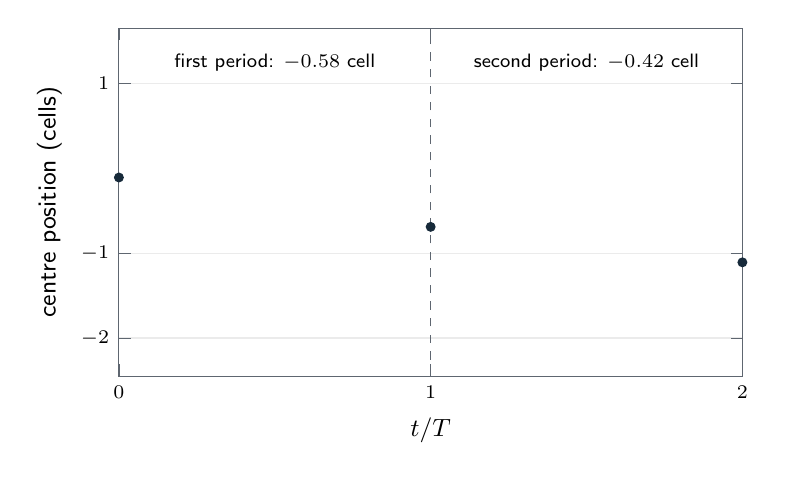
\begin{tikzpicture}
\begin{axis}[mbaxis,width=9.5cm,height=6cm,xmin=0,xmax=2,ymin=-2.45,ymax=1.65,clip=false,
  xlabel={$t/T$},ylabel={centre position (cells)},xtick={0,1,2},ytick={-2,-1,1},ymajorgrids,grid style={black!8}]
\FigDataComposite
\draw[dashed,rulegray] (axis cs:1,-2.45)--(axis cs:1,1.65);
\fill[ink] (axis cs:0,-0.109) circle (1.8pt);
\fill[ink] (axis cs:1,-0.691) circle (1.8pt);
\fill[ink] (axis cs:2,-1.109) circle (1.8pt);
\node[font=\scriptsize,anchor=south,fill=white,inner sep=1pt] at (axis cs:0.5,1.1) {first period: $-0.58$ cell};
\node[font=\scriptsize,anchor=south,fill=white,inner sep=1pt] at (axis cs:1.5,1.1) {second period: $-0.42$ cell};
\end{axis}
\end{tikzpicture}
\figtext{The followed orbital of Picture 2(b) in the question booklet (single-particle geometry at $K/J=-3/2$). Its first period moves it by about $-0.58$ cell and its second by about $-0.42$ cell. Only the sum, $-1$, is fixed by the two-cycle return, so $Q(0,T)$ and $Q(T,2T)$ need not each equal $-1/2$.}
\end{figpanel}


\begin{greenbox}{MFP [1] --- what the source supplies}
The source's branch-following argument connects two-period flavor winding to fractional average transport. A.1 isolates this counting step.
\end{greenbox}
\begin{redbox}{OPEN --- tracking was stipulated}
The argument has assumed actual following. It has not bounded excitation, internal mixing, or long-time transport error in a large interacting system.
\end{redbox}

\soltitle{A.2}{0.9}{A favorable domain need not form}
Each of the two interfaces changes one bond energy from $-J_z$ to $+J_z$. The interface cost is $4J_z$. Each of the $\ell$ flipped spins gains field energy $2h$:
\[
\boxed{\Delta E(\ell)=4J_z-2h\ell.}
\]
Strict negativity requires $\ell>2J_z/h$. Thus
\[
\boxed{\ell_{\min}=\left\lfloor\frac{2J_z}{h}\right\rfloor+1,}
\]
provided $\ell_{\min}\leq N-1$. If no such interior segment fits, this two-interface question has no allowed negative-energy segment.

At $g=0$, the Hamiltonian is diagonal in the $\sigma^z$ basis. The all-$A$ state is an eigenstate and acquires only a phase. It does not form a domain even when another configuration has lower energy.
\[
\boxed{\text{Energy preference is not a transition amplitude or a rate.}}
\]
\marking{Energy change: 0.3. Integer threshold and fit condition: 0.2. Stationary eigenstate and distinction from a rate: 0.4.}
\begin{figpanel}{A.2 --- domain energy (illustrative $J_z=1$, $h=0.45$)}
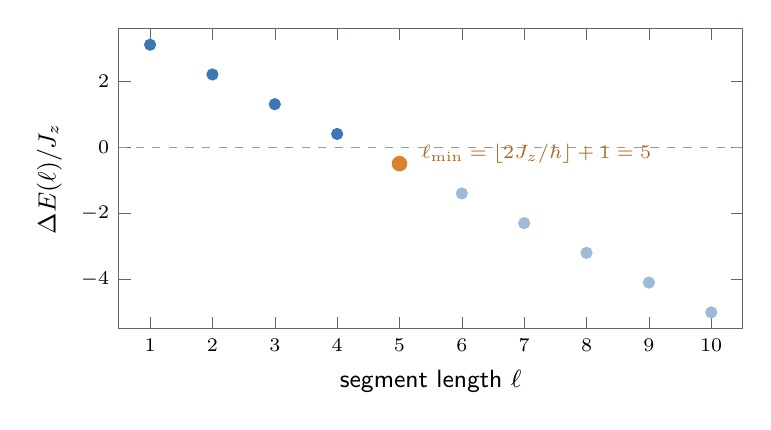
\begin{tikzpicture}
\begin{axis}[mbaxis,width=9.5cm,height=5.4cm,xmin=0.5,xmax=10.5,ymin=-5.5,ymax=3.6,xlabel={segment length $\ell$},ylabel={$\Delta E(\ell)/J_z$},xtick={1,...,10}]
\addplot[dashed,black!40,domain=0.5:10.5,forget plot] {0};
\addplot[only marks,mark=*,mark size=2pt,colB] coordinates {(1,3.1)(2,2.2)(3,1.3)(4,0.4)};
\addplot[only marks,mark=*,mark size=2.6pt,colA] coordinates {(5,-0.5)};
\addplot[only marks,mark=*,mark size=2pt,colB!50] coordinates {(6,-1.4)(7,-2.3)(8,-3.2)(9,-4.1)(10,-5.0)};
\node[font=\scriptsize,text=colA!80!black,anchor=west] at (axis cs:5.2,-0.2) {$\ell_{\min}=\lfloor 2J_z/h\rfloor+1=5$};
\end{axis}
\end{tikzpicture}
\figtext{$\Delta E(\ell)=4J_z-2h\ell$ decreases linearly; here $2J_z/h\approx4.44$. A negative $\Delta E$ only says the domain is lower in energy. With $g=0$ nothing in $H_{\rm d}$ can flip a spin, so the all-$A$ state stays where it is.}
\end{figpanel}

\begin{redbox}{ADDED MODEL --- scope of the answer}
This exact answer belongs to the teaching spin model. Deriving the domain variables, couplings, and driven transitions from MFP is a separate task.
\end{redbox}


\nextpage
\parttitle{M}{From the lattice to the geometric object}{1.0}
\bridgesol{M.1}{1.0}{Fourier transformation does not solve the interactions}
\textbf{(a)} The seam term becomes
\[
\sum_R c_{R+1,0}^\dagger c_{R,4}=\sum_k e^{-ik}c_{k,0}^\dagger c_{k,4}.
\]
Thus $H_0=\sum_k\bm c_k^\dagger h(k,\phi)\bm c_k$, with
\[
\boxed{
 h(k,\phi)=-\begin{pmatrix}
0&t_0&0&0&t_4e^{-ik}\\
t_0&0&t_1&0&0\\
0&t_1&0&t_2&0\\
0&0&t_2&0&t_3\\
t_4e^{ik}&0&0&t_3&0
\end{pmatrix}.}
\]
For real $k,\phi$ the hoppings are real and the seam entries are conjugate, so $h=h^\dagger$.

\textbf{(b)} From $Y^\dagger Y=\id_2$,
\[
p_{12}=YY^\dagger,\qquad p_{12}^2=p_{12},\qquad\Tr p_{12}=2.
\]
It is a rank-two single-particle projector in $\mathbb C^5$, or a point of $\operatorname{Gr}(2,5)$. The source's composite Wannier mechanism motivates choosing these bands. The choice is not made because a rank-two calculation is convenient.

\textbf{(c)} The three spaces are different:
\begin{center}\small
\begin{tabularx}{\textwidth}{@{}Y r@{}}\toprule
Restriction&Dimension at $N=4$\\\midrule
All $5N$ orbitals; only total particle number fixed&$\binom{20}{4}=4845$\\
Only the two composite bands; total particle number fixed&$\binom{8}{4}=70$\\
Two flavor orbitals per cell; exactly one occupied in every cell&$2^4=16$\\\bottomrule
\end{tabularx}
\end{center}
Translation-sector restrictions can reduce a dimension further; they are not included in this table. The single-particle Fourier transform leaves the physical interaction as a many-body operator. It does not make the full dynamics a $5\times5$ problem.

\marking{(a) Matrix with both seam entries and Hermiticity: 0.4. (b) Rank two in $\mathbb C^5$ and physical motivation: 0.3. (c) Three counts with their restrictions: 0.2; Fourier transformation leaves the interaction many-body: 0.1.}
\begin{greenbox}{DERIVATION --- exact change of representation}
The Fourier matrix and the dimension counts follow from the stated model and restrictions. They add a teaching connection, not a new MFP stability result.
\end{greenbox}
\handoff{Before extracting geometry, name the projector, its ambient space, and the physical reason for using it. Do not identify $p_{12}$ with a many-body low-energy pair.}

\nextpage
\parttitle{B}{Geometry and actual motion}{2.2}
\soltitle{B.1}{0.5}{The projector generator}
Differentiate $p^2=p$:
\[
\dot p\,p+p\dot p=\dot p.
\]
Multiply by $p$ on both sides. This gives $2p\dot p\,p=p\dot p\,p$, hence
\[
p\dot p\,p=0.
\]
Now
\[
\begin{split}
[[\dot p,p],p]
&=\dot p\,p-2p\dot p\,p+p\dot p\\
&=\dot p.
\end{split}
\]
Therefore $g_t=i[\dot p,p]$ obeys
\[
\boxed{[g_t,p]=i\dot p.}
\]
Since $[\dot p,p]$ is anti-Hermitian, $g_t$ is Hermitian. It is one generator of the prescribed subspace motion. It does not assert that the physical Hamiltonian produces the same tracking or internal occupation.
\marking{Differentiate and obtain $p\dot p\,p=0$: 0.2. Generator identity and interpretation: 0.3.}
\begin{greenbox}{H2 [2] --- exact kinematics}
The horizontal-generator construction applies to the given smooth projector. It does not supply the missing many-body dynamics or a transition rate.
\end{greenbox}

\soltitle{B.2}{0.9}{An exactly solvable moving frame}
The rotation gives
\[
W^\dagger HW=-\frac{\Delta}{2}\sigma_z,
\qquad -iW^\dagger\dot W=-\frac{\nu}{2}\sigma_y.
\]
Thus
\[
\boxed{\mathcal K=-\frac12(\Delta\sigma_z+\nu\sigma_y).}
\]
With $\omega=\sqrt{\Delta^2+\nu^2}$,
\[
e^{-i\mathcal Kt}=\id\cos\frac{\omega t}{2}
+i\frac{\Delta\sigma_z+\nu\sigma_y}{\omega}\sin\frac{\omega t}{2}.
\]
The instantaneous excited state is $W(t)\ket\downarrow$, so
\[
\boxed{P_{\rm ex}(t)=
\frac{\nu^2}{\Delta^2+\nu^2}
\sin^2\!\left(\frac{\sqrt{\Delta^2+\nu^2}\,t}{2}\right).}
\]
The path $p(t)$ has no $\Delta$ dependence, but the probability does. For $\Delta\gg\nu$ its maximum is small. The frame transformation has not removed the dynamics; it has made that dynamics explicit.
\marking{Moving-frame Hamiltonian: 0.35. Exact probability: 0.40. Same path, different tracking: 0.15.}
\begin{figpanel}{B.2 --- same projector path, different following}
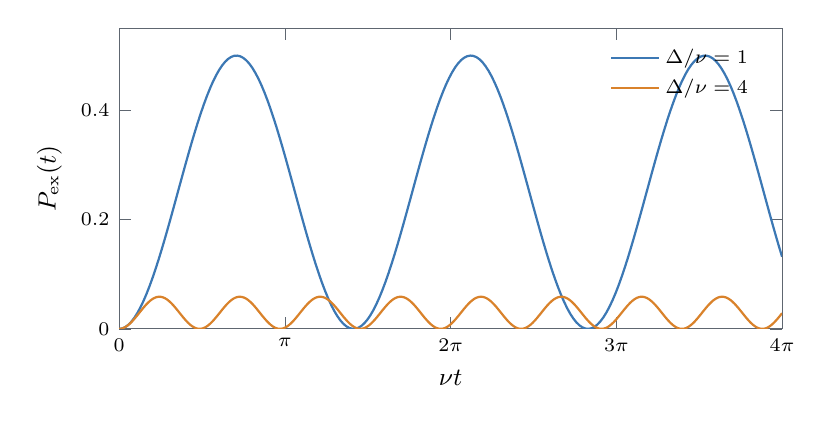
\begin{tikzpicture}
\begin{axis}[mbaxis,width=10cm,height=5.4cm,xmin=0,xmax=12.566,ymin=0,ymax=0.55,xlabel={$\nu t$},ylabel={$P_{\rm ex}(t)$},
  xtick={0,3.1416,6.2832,9.4248,12.566},xticklabels={$0$,$\pi$,$2\pi$,$3\pi$,$4\pi$},legend pos=north east]
\addplot[colB,thick,domain=0:12.566,samples=220] {sin(deg(sqrt(2)*x/2))^2/2};
\addplot[colA,thick,domain=0:12.566,samples=320] {sin(deg(sqrt(17)*x/2))^2/17};
\legend{$\Delta/\nu=1$,$\Delta/\nu=4$}
\end{axis}
\end{tikzpicture}
\figtext{$P_{\rm ex}=\frac{\nu^2}{\Delta^2+\nu^2}\sin^2\!\big(\tfrac12\sqrt{\Delta^2+\nu^2}\,t\big)$. The path $p(t)$ is identical in both curves; only $\Delta$ differs. A larger gap gives a smaller and faster oscillation.}
\end{figpanel}


\nextpage
\pagetitle{B.4 solution. Resolve the internal object}
\bridgesol{B.4}{0.8}{A gauge change is not a physical change of flavor}
\textbf{(a)} Since $\Lambda\Lambda^\dagger=\id_2$,
\[
(Y\Lambda)(Y\Lambda)^\dagger=YY^\dagger=p_{12}.
\]
For a fixed selected physical direction,
\[
(Y\Lambda)(\Lambda^\dagger v_A)(\Lambda^\dagger v_A)^\dagger(Y\Lambda)^\dagger
=Yv_Av_A^\dagger Y^\dagger=p_A.
\]
A compensated basis change alters only coordinates. Choosing a different direction in the plane without compensation changes the rank-one physical object. Arbitrary mixing of nondegenerate energy eigenvectors also means they are no longer individual energy eigenvectors; the composite space is still the same.

\textbf{(b)} One needs the Bloch eigenvectors, an internal localization prescription, and the physical position operator, including the orbital positions $r_s$. In a Wilson-loop implementation, the complete loop matrix around the Brillouin zone supplies internal eigenvectors and center phases with the appropriate basis sewing. One must unwrap and track the centers as $\phi$ changes. Degeneracies require an explicit continuation rule.

A Wilson loop around $k$ at fixed $\phi$ organizes Wannier centers. A geometric transport matrix along time organizes a chosen moving frame. The actual evolution uses $H(t)$ and its dynamical phases. These matrices must not be identified solely because all are unitary. The full projector family, spatial embedding, and localization rule can in principle define a flavor; endpoint closure alone cannot.

\textbf{(c)} The two supplied maps obey
\[
\det\id_2=1,\qquad\det(i\sigma_x)=i^2\det\sigma_x=1.
\]
But $\id_2$ keeps $A$ fixed, whereas $i\sigma_x\ket A=i\ket B$. Their determinant phases do not distinguish this action. Neither map includes a spatial displacement, so neither calculation alone proves a nonzero transported charge. A.1 required a separate center winding and actual following.

\marking{(a) Both invariances and the effect of an uncompensated choice: 0.3. (b) Required data; Wilson loop at fixed $\phi$ versus evolution in time: 0.3. (c) Equal determinants, different action, no displacement: 0.2.}
\begin{greenbox}{SOURCE CONNECTION --- where H2 enters}
MFP supplies a physical composite-band and Wannier construction. H2 organizes subspace motion and its internal-basis freedom. The bridge makes their objects explicit; it does not invent a new dynamical law.
\end{greenbox}
\begin{redbox}{OPEN --- not an automatic rank-one upgrade}
A closed composite projector does not certify the selected flavor's full internal rotation or seam. Nor does it prove that an interacting state occupies that branch over the drive. These are unchanged research conditions.
\end{redbox}
\handoff{Keep the full interactions when using the geometric frame. C.3 explains this step exactly.}

\nextpage
\parttitle{C}{Correlation in a single cluster}{3.9}
\soltitle{C.1}{1.2}{A two-channel correlated state}
The characteristic equation is $E^2-\Delta E-v^2=0$. The lower eigenvalue is
\[
\boxed{E_- =\frac{\Delta-\sqrt{\Delta^2+4v^2}}{2}.}
\]
A normalized lower eigenstate is
\[
\boxed{\ket{\psi_-}=\cos\vartheta\ket0-\sin\vartheta\ket d,
\qquad\tan2\vartheta=\frac{2v}{\Delta},\quad0<\vartheta<\frac\pi4.}
\]
For $v/\Delta\ll1$,
\[
\vartheta=\frac v\Delta+O\!\left(\frac{v^3}{\Delta^3}\right),
\quad E_-=-\frac{v^2}{\Delta}+O\!\left(\frac{v^4}{\Delta^3}\right),
\]
\[
|\braket d{\psi_-}|^2=\frac{v^2}{\Delta^2}
+O\!\left(\frac{v^4}{\Delta^4}\right).
\]
Thus a nonzero source may mainly dress the reference state rather than create a continually growing excitation population.

For evolution from $\ket0$, subtract the irrelevant term $(\Delta/2)\id$:
\[
H_X-\frac\Delta2\id=v\sigma_x-\frac\Delta2\sigma_z.
\]
Let $\omega_X=\sqrt{\Delta^2+4v^2}$. Exponentiating this Pauli matrix gives
\[
\boxed{P_d(t)=\frac{4v^2}{\Delta^2+4v^2}
\sin^2\!\left(\frac{\sqrt{\Delta^2+4v^2}\,t}{2}\right).}
\]
Therefore
\[
P_d(t)=v^2t^2+O(t^4).
\]
The exact probability oscillates and can return to zero. The initial curvature $v^2$ is not an irreversible decay rate.
\marking{Eigenvalue and state: 0.40. Weak-mixing forms: 0.25. Exact probability: 0.40. Rate distinction: 0.15.}
\begin{figpanel}{C.1 --- oscillation, not decay (illustrative $v/\Delta=0.3$)}
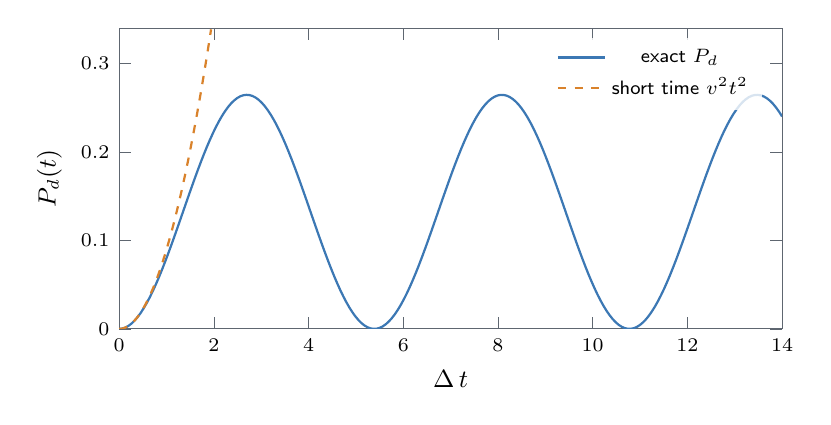
\begin{tikzpicture}
\begin{axis}[mbaxis,width=10cm,height=5.4cm,xmin=0,xmax=14,ymin=0,ymax=0.34,xlabel={$\Delta\, t$},ylabel={$P_d(t)$},legend pos=north east,legend style={fill=white,fill opacity=0.8,text opacity=1}]
\addplot[colB,thick,domain=0:14,samples=220] {0.36/1.36*sin(deg(sqrt(1.36)*x/2))^2};
\addplot[colA,thick,dashed,domain=0:1.94,samples=60] {0.09*x^2};
\legend{exact $P_d$,short time $v^2t^2$}
\end{axis}
\end{tikzpicture}
\figtext{The exact probability oscillates between $0$ and $4v^2/(\Delta^2+4v^2)$ and returns to zero. The short-time curvature $v^2$ describes only the start; it is not an irreversible decay rate.}
\end{figpanel}


\begin{greenbox}{GIVEN TOOL --- available source structure}
A two-body Hamiltonian acting on a Slater determinant produces single and double excitations. A one-body change of orbitals only supplies tangent single-excitation directions. Source strengths and rates are different quantities.
\end{greenbox}
\begin{redbox}{ADDED MODEL --- one channel is not a full spectrum}
The exact two-channel solution is not a fit of the full local response. A controlled reduction would need the actual channel energies, matrix elements, retained processes, and errors. The gap $\Delta$ in this page is a teaching parameter.
\end{redbox}

\nextpage
\parttitle{C}{Assembling neighboring corrections --- continued}{3.9}
\soltitle{C.2}{0.6}{Local improvement and new cross terms}
For the overlap diagnostic, commute only the operators on spin 2:
\[
\begin{aligned}
[h_{23},S_{12}]
&=-i\gamma\epsilon\,\sigma_1^x[\sigma_2^z,\sigma_2^x]\sigma_3^z\\
&=\boxed{2\gamma\epsilon\,\sigma_1^x\sigma_2^y\sigma_3^z.}
\end{aligned}
\]
This term acts on three sites. It was not present in the isolated 12-pair calculation. In fact, for real $\gamma,\epsilon$ its operator norm is $2|\gamma\epsilon|$.

A chain transformation combines overlapping corrections. Its transformed Hamiltonian contains cross commutators as well as the residual of each isolated cluster. It may also retain terms that change the reference configuration. Neither contribution can be discarded because the single-cluster residual decreased.
\marking{Commutator: 0.4. Why single-cluster success does not certify the chain: 0.2.}

\begin{redbox}{OPEN --- compatibility along the chain and drive}
A static correction at one phase does not provide a smooth full-cycle correction, its time derivative, or its two-cycle seam. Smaller isolated-cluster norms do not certify a small global or local interaction remainder after assembly.
\end{redbox}

\smallheading{Teacher's distinction}
There are three separate statements:
\begin{enumerate}[leftmargin=7mm,itemsep=5pt]
\item A particular pair has a more accurate correlated reference.
\item The pair corrections can be combined into a controlled chain description.
\item That description predicts the physical current during the full drive.
\end{enumerate}
A local calculation can supply the first statement; the second and third need separate work.


\nextpage
\pagetitle{C.3 solution. Exact rewriting versus approximation}
\bridgesol{C.3}{1.2}{Keep the Hamiltonian, the frame velocity, and the initial state}
\textbf{(a)} Differentiate $\ket\zeta=\mathcal U^\dagger\ket\Psi$ and use unitarity:
\[
i\partial_t\ket\zeta=\mathcal K_{\rm corr}\ket\zeta,\qquad
\mathcal K_{\rm corr}=\mathcal U^\dagger H_{\rm MFP}\mathcal U-i\mathcal U^\dagger\dot{\mathcal U}.
\]
Substitute $\mathcal U=We^S$:
\[
\boxed{\mathcal K_{\rm corr}=e^{-S}\mathcal K_W e^S
-i\int_0^1 e^{-uS}\dot S e^{uS}\,\dd u.}
\]
This is exact for any specified differentiable unitary frame and anti-Hermitian $S$.

\textbf{(b)} Expansion gives
\[
\begin{split}
\mathcal K_{\rm corr}={}&\mathcal K_W+[\mathcal K_W,S]-i\dot S\\
&+\tfrac12[[\mathcal K_W,S],S]-\tfrac i2[\dot S,S]+\cdots.
\end{split}
\]
The first line contains all first-order terms in the stated expansion. The frame's velocity contributes even when a static transformation reduces a residual at one phase. A static result alone does not bound $\dot S$ throughout a cycle.

\textbf{(c)} The equality $\mathcal K_{\rm corr}=\mathcal K_{\rm ret}+\mathcal R$ is only a partition. An approximation occurs when $\mathcal R$ is omitted or replaced. The exact physical initial density matrix becomes
\[
\rho'(0)=\mathcal U^\dagger(0)\rho(0)\mathcal U(0).
\]
Choosing a projected or simpler reference state instead adds an initial-state error. It is not a consequence of the basis transformation. A useful reduced calculation must bound the effect of $\mathcal R$, not just rename it.

\textbf{(d)} A one-particle rotation replaces each $c_j$ by a linear combination of modes. A quartic interaction remains a sum of quartic terms, generally with more orbital indices. No high band has been removed by this operation. The displayed $e^S$ specifies the form of a possible many-body dressing, not its values or its spatial decay.

\marking{(a) Exact generator: 0.4. (b) First-order terms and the role of $\dot S$: 0.3. (c) Where the approximation enters, transformed initial state, need for a bound: 0.3. (d) Interaction stays two-body; $e^S$ unspecified: 0.2.}
\begin{greenbox}{DERIVATION}
The exact product-frame formula and the explicit initial-state transformation connect the existing geometric and current identities. Their algebra is not a new MB1 lifetime computation.
\end{greenbox}
\begin{redbox}{OPEN --- a useful retained model}
One must still choose and solve $\mathcal K_{\rm ret}$, control the omitted terms and observables, and retain any physical mixing that changes the current. A small model error does not imply a perfectly quantized reference pump.
\end{redbox}

\nextpage
\pagetitle{C.4 solution. A remainder is not the whole story}
\bridgesol{C.4}{0.9}{The retained dynamics can change the state}
\textbf{(a)} The fixed direction is preserved up to a phase if and only if, for every time in the interval,
\[
\boxed{(1-\Pi_A)\mathcal K_{\rm ret}(t)\ket{A_0}=0.}
\]
Equivalently $\mathcal K_{\rm ret}(t)\ket{A_0}=E_A(t)\ket{A_0}$. Then its solution is $e^{-i\int E_A\,dt}\ket{A_0}$. This statement concerns a fixed direction in the chosen frame; a moving reference needs its frame-velocity term.

\textbf{(b)} In the periodic teaching chain, the diagonal part gives $E_A=-NJ_z+Nh$. The transverse field gives
\[
\boxed{(H_{\rm d}-E_A)\ket{A_0}=-g\sum_{j=1}^{N}\ket j.}
\]
The $\ket j$ are mutually orthogonal, hence
\[
\norm{(H_{\rm d}-E_A)\ket{A_0}}^2=Ng^2.
\]
For a given cell, the first-order amplitude of its single flip is $igt$, and
\[
\boxed{\langle q_j(t)\rangle=g^2t^2+O(t^3).}
\]
The global source norm grows with $N$, while this local initial coefficient does not. This is a short-time expansion, not a uniform long-time estimate.

\textbf{(c)} By construction, $\mathcal K_{\rm ret}$ is the exact Hamiltonian of this teaching example and $\mathcal R=0$. There is no truncation error, yet the retained dynamics changes the reference direction. Model accuracy and reference-pump stability are different questions. No physical MFP current has been specified or evaluated here, so there is no MFP lifetime result.

\marking{(a) Invariance condition: 0.2. (b) Source vector 0.2, norm $Ng^2$ 0.1, $\langle q_j\rangle=g^2t^2$ 0.2. (c) The three distinctions: 0.2.}
\begin{redbox}{ADDED MODEL --- what the exact answer does not establish}
The spin example is only a counterexample to the claim that zero omitted remainder implies no physical evolution. Its $g^2$ coefficient cannot be inserted into F.1 as an MB1 error-growth bound.
\end{redbox}
\handoff{Predict $\ket\Xi$ or its relevant local reduced states. Do not first impose ideal charge on a reference whose retained dynamics has not been solved.}

\nextpage
\parttitle{D}{Current and phase}{2.0}
\soltitle{D.1}{0.6}{The same probability can give opposite currents}
Let $a=\sqrt{1-p}$ and $b=e^{i\beta}\sqrt p$. Then
\[
\begin{aligned}
\langle I\rangle
&=-i\lambda\,a^*b+i\lambda\,b^*a\\
&=\boxed{2\lambda\sqrt{p(1-p)}\sin\beta.}
\end{aligned}
\]
Thus the three requested phases give
\[
\begin{array}{c|ccc}
\beta&0&\pi/2&-\pi/2\\\hline
\langle I\rangle&0&2\lambda\sqrt{p(1-p)}&-2\lambda\sqrt{p(1-p)}
\end{array}
\]
For small $p$ and a fixed nonzero $\sin\beta$, the leading magnitude is proportional to $\sqrt p$. A probability contains no information about the relative phase $\beta$ and does not determine the current.
\marking{Expectation value: 0.35. Phase comparison and scaling: 0.15. Probability alone is insufficient: 0.10.}
\begin{figpanel}{D.1 --- the current follows the phase}
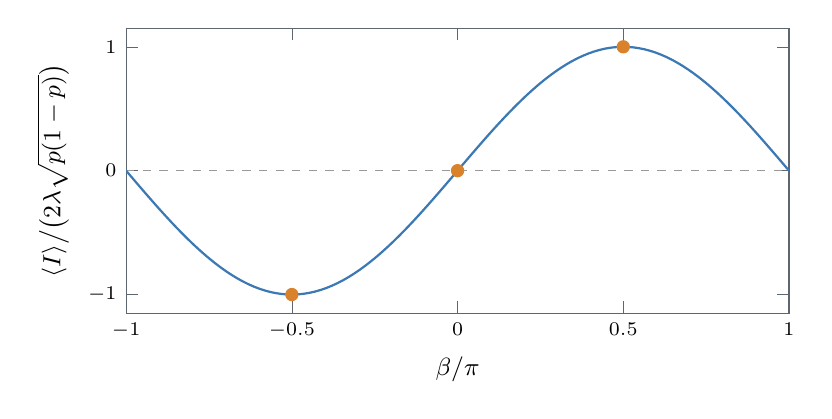
\begin{tikzpicture}
\begin{axis}[mbaxis,width=10cm,height=5.2cm,xmin=-1,xmax=1,ymin=-1.15,ymax=1.15,xlabel={$\beta/\pi$},ylabel={$\langle I\rangle\big/\big(2\lambda\sqrt{p(1-p)}\big)$},xtick={-1,-0.5,0,0.5,1}]
\addplot[dashed,black!40,domain=-1:1,forget plot] {0};
\addplot[colB,thick,domain=-1:1,samples=120] {sin(180*x)};
\addplot[only marks,mark=*,colA,mark size=2.2pt] coordinates {(-0.5,-1)(0,0)(0.5,1)};
\end{axis}
\end{tikzpicture}
\figtext{$\langle I\rangle=2\lambda\sqrt{p(1-p)}\sin\beta$. The same $p$ gives zero, positive or negative current depending on $\beta$; at small $p$ the size scales as $\sqrt p$.}
\end{figpanel}


\smallheading{Why the current-connected state is not automatically a double excitation}
A hopping current has the one-body form
\[
I=\sum_{ab}I_{ab}d_a^\dagger d_b.
\]
It changes at most one occupied orbital of a Slater determinant. If $\ket{\Phi_{ij}^{ab}}$ differs from $\ket\Phi$ by two occupied orbitals, then
\[
\bra{\Phi_{ij}^{ab}}I\ket\Phi=0.
\]
A double-excitation source can still influence later dynamics and the current of a correlated state. The vanishing direct matrix element only forbids identifying every source norm with the two-state current amplitude $\lambda$.

\begin{redbox}{ADDED MODEL --- the current matrix is part of the question}
D.1 assumes a current-connected pair. The example isolates interference. It does not specify how the physical MFP evolution generates that pair or its phase.
\end{redbox}
\begin{greenbox}{INTERPRETATION --- a useful distinction}
A static correlation correction and a dynamical phase correction have different roles. The physical current must be evaluated with the actual operators and state. An external-state probability or a domain count cannot replace it.
\end{greenbox}

\nextpage
\parttitle{D}{The exact physical-current transformation --- continued}{2.0}
\soltitle{D.2}{1.4}{A frame-dependent Hamiltonian derivative is incomplete}
Write $H'=\mathcal U^\dagger H\mathcal U$. From unitarity,
\[
\partial_\theta H'
=\mathcal U^\dagger(\partial_\theta H)\mathcal U
+i[\mathcal A_\theta,H'].
\]
Since $I=-\partial_\theta H$,
\[
I'=-\partial_\theta H'+i[\mathcal A_\theta,H'].
\]
Substitute $H'=\mathcal K+\mathcal A_t$:
\[
I'=-\partial_\theta \mathcal K-\partial_\theta\mathcal A_t
+i[\mathcal A_\theta,\mathcal K]+i[\mathcal A_\theta,\mathcal A_t].
\]
Use the supplied connection identity to cancel the last commutator. The result is
\[
\boxed{I'=-\partial_\theta \mathcal K-\partial_t\mathcal A_\theta
-i[\mathcal K,\mathcal A_\theta].}
\]
For $i\partial_t\ket\Xi=\mathcal K\ket\Xi$,
\[
\frac{\dd}{\dd t}\langle\mathcal A_\theta\rangle
=\left\langle\partial_t\mathcal A_\theta+i[\mathcal K,\mathcal A_\theta]\right\rangle.
\]
Integrating the physical current therefore gives
\[
\boxed{
Q(t_1,t_2)
=-\int_{t_1}^{t_2}\langle\partial_\theta \mathcal K\rangle\,\dd t
-\big[\langle\mathcal A_\theta\rangle\big]_{t_1}^{t_2}.
}
\]
All expectation values here use the same transformed physical state. If more than one gauge patch is used, patch seams must be included consistently.

A closed projector path fixes a subspace, not a unique frame or its holonomy. It does not imply that the endpoint term vanishes. The two terms are frame-dependent; their sum is the physical charge. In particular, the endpoint term alone is not automatically a Chern charge.
\marking{Differentiate $H'$ and obtain the operator identity: 0.8. Integrate using the equation of motion: 0.4. Endpoint and gauge interpretation: 0.2.}

\begin{greenbox}{EXACT IDENTITY}
This result is an exact change of representation. It does not require weak interactions, a small residual, or a short drive period. It can therefore be used to check a proposed reduction without changing the original physical current.
\end{greenbox}
\begin{redbox}{OPEN --- solving the expectation values}
The full research problem still needs the driven correlated state, the physical current in that state, and the correct reference charge. Rewriting the current is not yet predicting it.
\end{redbox}

\nextpage
\parttitle{E}{A local observable does not require global fidelity}{2.4}
\soltitle{E.1}{0.5}{A product-state diagnostic}
The global overlap amplitude is $(\sqrt{1-p})^N$, so
\[
\boxed{\mathcal F_N=(1-p)^N.}
\]
The reduced state of $m$ cells is still the prescribed product state:
\[
\boxed{\mathcal F_m=(1-p)^m.}
\]
For fixed $p>0$, $\mathcal F_N\to0$ as $N\to\infty$, but $\mathcal F_m$ is independent of the rest of the chain. Poor global overlap alone cannot diagnose a large error in a fixed local observable. It also does not prove local transport stability.
\marking{Global fidelity: 0.2. Local fidelity: 0.2. Correct interpretation: 0.1.}
\begin{figpanel}{E.1 --- global versus local fidelity (illustrative $p=0.05$, $m=3$)}
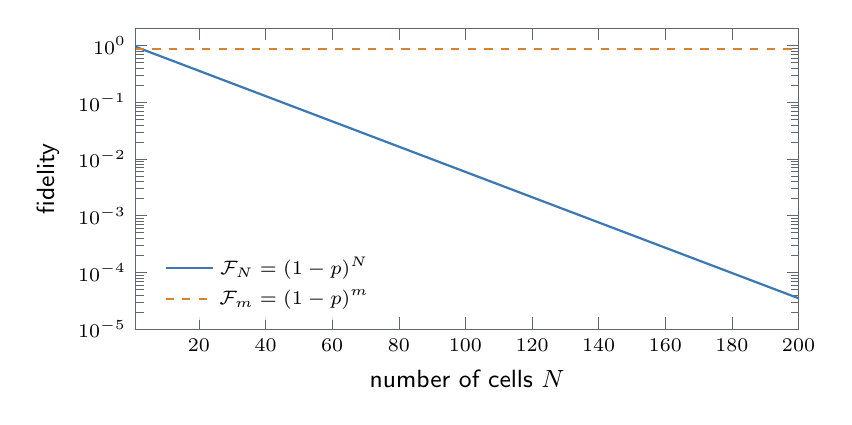
\begin{tikzpicture}
\begin{axis}[mbaxis,width=10cm,height=5.4cm,ymode=log,xmin=1,xmax=200,ymin=1e-5,ymax=2,xlabel={number of cells $N$},ylabel={fidelity},legend pos=south west,legend style={fill=white,fill opacity=0.8,text opacity=1}]
\addplot[colB,thick,domain=1:200,samples=120] {0.95^x};
\addplot[colA,thick,dashed,domain=1:200,samples=2] {0.857375};
\legend{$\mathcal F_N=(1-p)^N$,$\mathcal F_m=(1-p)^m$}
\end{axis}
\end{tikzpicture}
\figtext{The global fidelity decays exponentially with $N$, while the fidelity of a fixed window does not change. A tiny global overlap says nothing, by itself, about a local current.}
\end{figpanel}


\soltitle{E.2}{1.0}{A trace-distance bound for the current}
Write
\[
\Delta I=\Tr[(\rho'-\sigma')I_X]+
\Tr[(\rho'-\sigma')(I'-I_X)].
\]
The first term depends only on the states reduced to $X$. Apply the supplied norm inequalities:
\[
\boxed{|\Delta I|\leq\norm{I_X}\norm{\rho'_X-\sigma'_X}_1+2\eta_X.}
\]
For a product reference, define $P_X=\ket{A_{0,X}}\bra{A_{0,X}}=\prod_{x\in X}(1-q_x)$. Since $1-P_X\leq\sum_xq_x$,
\[
1-\Tr(\rho'_X P_X)\leq D_X.
\]
The pure-state trace-distance inequality, together with its maximum value 2, gives
\[
\norm{\rho'_X-P_X}_1\leq2\min(1,\sqrt{D_X}).
\]
Hence
\[
\boxed{|\Delta I|\leq2\norm{I_X}\min(1,\sqrt{D_X})+2\eta_X.}
\]
For a general correlated reference, use the first trace-distance bound. Do not impose the product-reference expression for $D_X$ without a justified frame and factorization.
\marking{General current bound: 0.5. Product-reference bound: 0.4. Scope and interpretation: 0.1.}

\begin{greenbox}{CONDITIONAL ERROR CONTROL}
The observable bound does not contain a factor proportional to the total number of cells. Its usefulness depends on the local trace distance, current norm, and spatial-tail estimate.
\end{greenbox}
\begin{redbox}{OPEN --- the unknown dynamical input}
The inequality does not predict $\rho'_X-\sigma'_X$. Nor does it prove that $D_X$ is a domain density or a decay rate. Establishing a useful full-cycle bound on these quantities remains part of the research.
\end{redbox}

\nextpage
\pagetitle{E.3 solution. Locality does not close the state equation}
\bridgesol{E.3}{0.9}{The boundary correlations carry dynamical information}
\textbf{(a)} Take the partial trace of the reference equation. Since $\mathcal K_X$ acts inside $X$,
\[
\Tr_{\bar X}[\mathcal K_X,\sigma']=[\mathcal K_X,\sigma'_X].
\]
Cyclicity for exterior operators gives $\Tr_{\bar X}[\mathcal K_{\bar X},\sigma']=0$. Thus
\[
\boxed{
i\dot\sigma'_X=[\mathcal K_X,\sigma'_X]
+\Tr_{\bar X}[\mathcal K_{\partial X},\sigma'].
}
\]

\textbf{(b)} The last term generally depends on the state across the boundary, not on $\sigma'_X$ alone. Even a short-range boundary Hamiltonian needs correlations with the nearby exterior. Under evolution those correlations can depend on farther degrees of freedom. A larger cluster, a controlled approximation, or a suitable error estimate is needed. The composite single-particle gap controls a different object; it does not specify this many-body correlation term.

\textbf{(c)} Subtract the two full equations:
\[
\boxed{
i\partial_t\delta\rho
=[\mathcal K_{\rm ret},\delta\rho]+[\mathcal R,\rho'].
}
\]
Its initial value is
\[
\delta\rho(0)=\mathcal U^\dagger(0)\rho(0)\mathcal U(0)-\sigma'(0).
\]
The first term propagates existing differences. The second contains the effect of omitted dynamics on the actual state. The identity is exact, but $\rho'$ is not thereby known. Taking a partial trace does not remove the need for correlation information or a controlled estimate of this term.

\marking{(a) Local equation, with the exterior term vanishing: 0.35. (b) Boundary correlations needed; the band gap does not supply them: 0.25. (c) Difference equation, initial value, not yet a bound: 0.3.}
\begin{greenbox}{DERIVATION --- where the missing input belongs}
The local state equation and difference equation follow from the two specified dynamical equations. They locate the input needed by E.2. They are not a solved local closure for MFP.
\end{greenbox}
\begin{redbox}{OPEN --- preserve the initial state and the model}
A nonzero initial difference cannot be set to zero by renormalizing a projected state. An assumed bath or factorization changes the approximation and needs its own justification. A local norm estimate must remain useful over the time interval and as the chain grows.
\end{redbox}
\handoff{The project must compute a physical reference charge and a usable error, not only a geometric trajectory. F.3 gives the conditional decision rule without assigning an ideal charge to the reference.}

\nextpage
\parttitle{F}{A certificate, not an exact lifetime}{1.5}
\soltitle{F.1}{0.7}{Integrating the supplied local bounds}
The given inequality includes $s=0$, hence requires $D_X(0)=0$. This is a classroom premise. Under the full stated hypothesis, $\min(1,\sqrt{D_X(s)})\leq\alpha s$ for $s\geq0$, and E.2 gives
\[
|\Delta I(s)|\leq2I_0\alpha s+2\eta.
\]
Integrate over a two-period window:
\[
\begin{aligned}
|\Qbar-\Qbar_{\rm ref}|
&\leq\frac12\int_{t-2T}^{t}(2I_0\alpha s+2\eta)\,\dd s\\
&=2I_0\alpha T(t-T)+2T\eta.
\end{aligned}
\]
Add the supplied reference-charge error:
\[
\boxed{|\Qbar(t)-Q_*|\leq\delta_0+2I_0\alpha T(t-T)+2T\eta.}
\]
For $\alpha I_0>0$, an algebraic endpoint is
\[
\boxed{t_{\rm cert}=T+\frac{\delta-\delta_0-2T\eta}{2I_0\alpha T}.}
\]
Require $\delta-\delta_0-2T\eta>0$. The useful certified interval is
\[
2T\leq t\leq\min(t_{\max},t_{\rm cert}),
\]
and it is nonempty only if this upper endpoint is at least $2T$.

For the numerical exercise, express time in $\tau_0=T$. Then
\[
\frac{t_{\rm cert}}{T}
=1+\frac{0.005-0.001-0.00002}{0.00002}
=\boxed{200}.
\]
The assumptions were stipulated to hold until $201T$. Thus all stated windows ending from $2T$ through $200T$ are certified. The next period need not fail: the bound has merely stopped certifying it.
\marking{Integrated bound: 0.25. Endpoint and conditions: 0.20. Numerical value: 0.15. Lower-bound interpretation: 0.10.}
\begin{figpanel}{F.1 --- where the certificate ends}
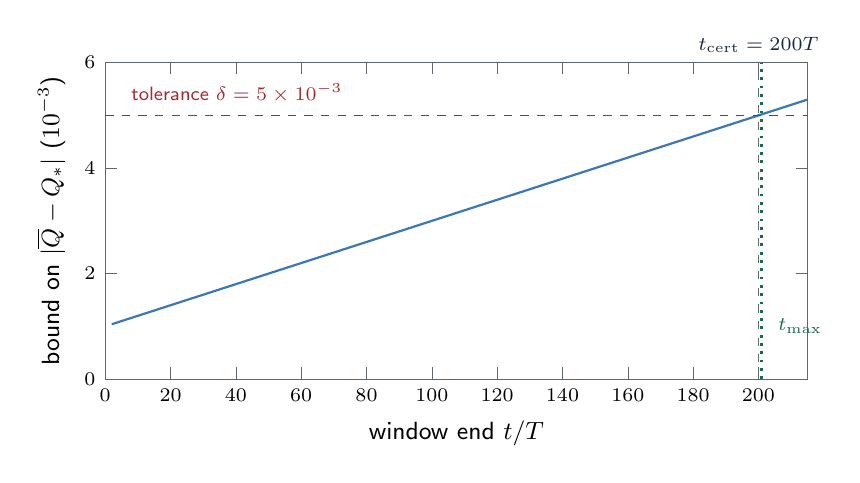
\begin{tikzpicture}
\begin{axis}[mbaxis,width=10.5cm,height=5.6cm,xmin=0,xmax=215,ymin=0,ymax=6,xlabel={window end $t/T$},ylabel={bound on $|\Qbar-Q_*|$ ($10^{-3}$)},clip=false]
\addplot[colB,thick,domain=2:215,samples=2] {1.02+0.02*(x-1)};
\addplot[openred,dashed,domain=0:215,samples=2] {5};
\draw[dashed,rulegray] (axis cs:200,0)--(axis cs:200,6) node[above,font=\scriptsize,text=ink]{$t_{\rm cert}=200T$};
\draw[dotted,sourcegreen,line width=1pt] (axis cs:201,0)--(axis cs:201,6);
\node[font=\scriptsize,text=openred,anchor=south west] at (axis cs:5,5.05) {tolerance $\delta=5\times10^{-3}$};
\node[font=\scriptsize,text=sourcegreen,anchor=west] at (axis cs:203,1) {$t_{\max}$};
\end{axis}
\end{tikzpicture}
\figtext{The bound $\delta_0+2T\eta+2I_0\alpha T(t-T)$ grows linearly and reaches $\delta$ at $t=200T$. After that the bound no longer certifies anything; it does not predict a failure.}
\end{figpanel}

\begin{redbox}{ILLUSTRATIVE ONLY --- no MB1 lifetime has been computed}
The value $200T$ follows from illustrative classroom inputs. The complete correlated-frame bounds, their common time interval, and the required initial matching have not been established for MB1.
\end{redbox}

\smallheading{Connection to C.4}
The product-reference form of E.2 uses $\sigma'_X=\ket{A_{0,X}}\bra{A_{0,X}}$ at every time $s$ in the window. This is consistent only if the kept dynamics leaves the reference direction invariant, which is the C.4(a) condition
\[
(1-\Pi_A)\,\mathcal K_{\rm ret}(s)\ket{A_0}=0\qquad(0\le s\le t_{\max}),
\]
together with the frame-velocity term if the reference direction moves. C.4(b) gives a counterexample with $\mathcal R=0$: the source $-g\sum_j\ket j$ moves the reference at order $t$. When the condition fails, $D_X$ measured against a fixed $\ket{A_{0,X}}$ no longer measures $\rho'_X-\sigma'_X$. Use the general bound $\norm{I_X}\norm{\rho'_X-\sigma'_X}_1+2\eta_X$ with the evolving reference, and compute $\Qbar_{\rm ref}$ from that reference as in F.3. A student who notes this restriction in F.1 deserves credit under ``conditions''.

\nextpage
\pagetitle{F.3 solution. A reference can itself fail}
\bridgesol{F.3}{0.8}{Use intervals, not an unqualified platform label}
\textbf{(a)} Integration gives the computable candidate budget
\[
\boxed{E(t)=\frac12\int_{t-2T}^{t}
\big[b_X(s)e_X(s)+2\eta(s)\big]\,\dd s.}
\]
Then $|\Qbar-\widehat Q|\leq E$ if all supplied bounds hold on the window. The local-state estimate $e_X$ must include any initial mismatch. If the reference charge is evaluated with a truncated operator or an approximate integrator, its additional error must also be included; the definition here used the full $I'$.

\textbf{(b)} The triangle inequality and its reverse give
\[
\begin{array}{ll}
|\widehat Q-Q_*|+E\leq\delta&\Rightarrow\text{certified inside},\\[3pt]
|\widehat Q-Q_*|-E>\delta&\Rightarrow\text{certified outside}.
\end{array}
\]
If neither holds, the classification is undetermined. The second inequality is strict because equality still satisfies the specified tolerance.

\textbf{(c)} For the supplied arithmetic,
\begin{center}\small
\begin{tabular}{@{}lrrl@{}}\toprule
Window&$|\widehat Q-Q_*|+E$&$|\widehat Q-Q_*|-E$&Decision\\\midrule
1&0.0040&0.0020&Inside\\
2&0.0075&0.0045&Undetermined\\
3&0.0065&0.0055&Outside\\\bottomrule
\end{tabular}
\end{center}
The first failed window among these three samples may be 2 or 3. The data do not decide which. Windows at unlisted start times are uncontrolled, so the first continuous-start failure is not determined. A different persistence rule would require additional consecutive-window information.

\begin{figpanel}{F.3 --- three sample windows}
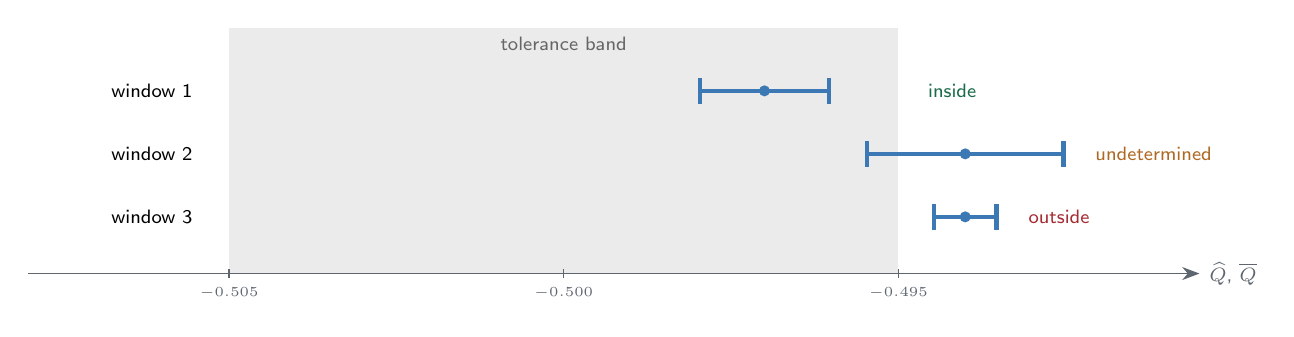
\begin{tikzpicture}[x=8.5mm,y=8mm]
\fill[black!8] (2,-0.4) rectangle (12,3.5);
\draw[->,rulegray] (-1,-0.4)--(16.5,-0.4) node[right,font=\scriptsize]{$\widehat Q$, $\Qbar$};
\foreach \x/\l in {2/{-0.505},7/{-0.500},12/{-0.495}}{\draw[rulegray] (\x,-0.33)--(\x,-0.47) node[below,font=\tiny]{$\l$};}
\node[font=\scriptsize,text=black!60] at (7,3.25) {tolerance band};
% window 1: -0.497 +- 0.001 -> x = 7 + (Q+0.5)*1000
\draw[colB,line width=1.6pt,|-|] (9,2.5)--(11,2.5); \fill[colB] (10,2.5) circle (2pt);
\node[font=\scriptsize,anchor=east] at (1.6,2.5) {window 1};
\node[font=\scriptsize,anchor=west,text=sourcegreen] at (12.3,2.5) {inside};
\draw[colB,line width=1.6pt,|-|] (11.5,1.5)--(14.5,1.5); \fill[colB] (13,1.5) circle (2pt);
\node[font=\scriptsize,anchor=east] at (1.6,1.5) {window 2};
\node[font=\scriptsize,anchor=west,text=colA!80!black] at (14.8,1.5) {undetermined};
\draw[colB,line width=1.6pt,|-|] (12.5,0.5)--(13.5,0.5); \fill[colB] (13,0.5) circle (2pt);
\node[font=\scriptsize,anchor=east] at (1.6,0.5) {window 3};
\node[font=\scriptsize,anchor=west,text=openred] at (13.8,0.5) {outside};
\end{tikzpicture}
\figtext{Each bar is $\widehat Q\pm E$. Window 1 lies wholly inside the band, window 3 wholly outside, and window 2 straddles the edge, so it is undetermined. Whether window 2 or 3 is the first failure cannot be decided from these data.}
\end{figpanel}

\marking{(a) $E(t)$ and where the initial mismatch enters: 0.3. (b) Both tests and the undetermined case: 0.3. (c) Classification and undetermined first failure: 0.2.}
\begin{redbox}{ADDED DATA --- no lifetime result}
These decisions follow from supplied numerical error budgets. They are not evidence that an MFP simulation passed or failed at these times. The $200T$ example in F.1 remains an independent classroom calculation.
\end{redbox}
\begin{greenbox}{LOGIC --- preserve the final research goal}
A useful reference predicts $\widehat Q(t)$; it need not remain ideal forever. Error control can then certify a stable interval or an actual failed window. Predicting first failure and its physical mechanism requires control of the preceding dynamics as well.
\end{greenbox}

\nextpage
\parttitle{X}{Synthesis: what would a prediction need?}{0.5}
\soltitle{X.1}{0.5}{The missing inputs are the research}
\begin{redbox}{OPEN --- no standard numerical answer is claimed}
The scored exercise supplied several assumptions. The paper must derive suitable replacements from the microscopic MFP model and a specified physical initial state. The final task is not another substitution into the classroom formula.
\end{redbox}

A candidate description has the structure
\[
\ket{\Psi_{\rm ref}(t)}=W(t)e^{S(t)}\ket{\Xi(t)}.
\]
Here $W$ follows a geometric reference frame, $S$ supplies correlation corrections, and $\ket\Xi$ retains physical configuration mixing. If the retained Hamiltonian changes the reference direction, $\ket\Xi$ cannot be replaced by one overall phase.

\smallheading{What must be supplied by the research model}
\begin{enumerate}[leftmargin=7mm,itemsep=5pt]
\item A reference defined without using the unknown exact long-time state, with controlled locality, time dependence, and two-period seams.
\item A description of retained correlated dynamics and of all omitted effects. Higher-band terms and overlapping corrections must be included or bounded.
\item A physical-current prediction, with the correct transformed operator, initial state, and boundary terms.
\item A useful local error estimate over complete cycles. It must distinguish an upper bound from a fitted error curve.
\end{enumerate}

If the final result has the form
\[
|\Qbar(t)-\widehat Q(t)|\leq E(t),
\]
then the triangle inequality and reverse triangle inequality give
\[
\begin{array}{ll}
|\widehat Q-Q_*|+E\leq0.005
&\Longrightarrow\text{window certified to pass},\\[3pt]
|\widehat Q-Q_*|-E>0.005
&\Longrightarrow\text{window certified to fail}.
\end{array}
\]
Neither implication, by itself, locates the first failure. Earlier windows, any persistence rule, and gaps between sampled start times need control.

\marking{Reference with controlled seams: 0.1. Kept dynamics and omitted effects: 0.1. Physical-current prediction: 0.1. Useful local error over full cycles: 0.1. First failure needs earlier windows, any persistence rule and gaps between starts: 0.1.}
\begin{greenbox}{SUMMARY --- what has been reduced to precise statements}
The source mechanism and projector identity are supplemented by exact frame, current and local-error identities. The full-cycle correlated reference, its actual current, and a useful time-uniform local-error estimate are still not established.
\end{greenbox}
\begin{redbox}{OPEN --- lower bounds versus actual failure}
A guaranteed operating interval and a prediction of actual first failure are different outputs. A small static source, a source norm, or a single favorable domain energy is not sufficient for either one without the missing dynamics and current analysis.
\end{redbox}

\nextpage
\pagetitle{Teacher notes for the public example}
\smallheading{What this example is}
A public excerpt of a 26-question, 20-point guided problem (Revision 4). The questions that used unpublished project calculations or proofs (B.3, B.G1, B.G2, R.1, R.2, E.G1, E.G2, F.2) were removed; the other 18 questions and their marks are unchanged except C.2 (the part on reported data was removed, 0.6 pt) and X.1 (0.5 pt). Labels were kept, so they are not consecutive.

\smallheading{Notation}
$K$ is only the modulation amplitude; generators are calligraphic ($\mathcal K$). $Y$ is the eigenvector matrix, $\Lambda$ a $2\times2$ unitary, $\mathcal F$ a fidelity, $\gamma$ the coupling in $h_{23}$, $\lambda$ the current matrix element, $I_X$ the local current, $\id$ the identity.

\smallheading{The computed pictures and a sign observation}
\texttt{figures.py} computes the band pictures from $h(k,\phi)$ and the Wannier centres from the projected position operator $Pe^{2\pi ix/L}P$ on a 24-cell ring at $K/J=-3/2$. With the Hamiltonian exactly as printed in [1], orbitals of band 1 move by $+2$ cells per period, and the followed composite flavor moves by $-1$ cell in two periods. An explicit time evolution of the filled band 1 on a 12-cell ring ($T=400/J$) gives a rightward charge of $+2.00$ per period through every bond. These signs agree with the values $Q=+2$ and $Q=-1/2$ in Fig.~4 of [1] if $Q$ is counted rightward-positive, as in this problem. For this Hamiltonian, the current expression printed in [1], $i\langle J_jc_j^\dagger c_{j+1}-J_jc_{j+1}^\dagger c_j\rangle$, is minus the rightward bond current, so [1] presumably uses a convention not stated there.

\nextpage
\pagetitle{Sources}
\sourceentries
\vfill
\begin{center}\textbf{End of solution booklet}\end{center}
\end{document}
